\documentclass[11pt,a4paper]{article}
\usepackage[T1]{fontenc}
\usepackage[utf8]{inputenc}
\usepackage[margin=1in]{geometry}
\usepackage{lmodern,microtype}
\usepackage{amsmath,amssymb,amsthm,mathtools}
\usepackage{enumitem,booktabs,array}
\usepackage{tikz}
\usetikzlibrary{arrows.meta}
\usepackage{xurl}
\usepackage[dvipsnames]{xcolor}
\usepackage[colorlinks=true,linkcolor=MidnightBlue,citecolor=MidnightBlue,
  urlcolor=MidnightBlue]{hyperref}
\usepackage[capitalise,noabbrev,nameinlink]{cleveref}
\usepackage{bookmark}
\usepackage{accsupp,letltxmacro}
\usepackage{needspace}
\pdfinfoomitdate=1
\pdftrailerid{}
\pdfsuppressptexinfo=15
\input{glyphtounicode}
\input{glyphtounicode-cmex}
\pdfgentounicode=1
\LetLtxMacro{\KSOriginalMapsto}{\mapsto}
\LetLtxMacro{\KSOriginalHookrightarrow}{\hookrightarrow}
\renewcommand{\mapsto}{%
  \BeginAccSupp{pdfliteral=direct,method=hex,unicode,ActualText=21A6}%
  \KSOriginalMapsto\EndAccSupp{pdfliteral=direct}}
\renewcommand{\hookrightarrow}{%
  \BeginAccSupp{pdfliteral=direct,method=hex,unicode,ActualText=21AA}%
  \KSOriginalHookrightarrow\EndAccSupp{pdfliteral=direct}}
\LetLtxMacro{\KSOriginalNe}{\ne}
\renewcommand{\ne}{%
  \BeginAccSupp{pdfliteral=direct,method=hex,unicode,ActualText=2260}%
  \KSOriginalNe\EndAccSupp{pdfliteral=direct}}
\LetLtxMacro{\KSOriginalNotin}{\notin}
\renewcommand{\notin}{%
  \BeginAccSupp{pdfliteral=direct,method=hex,unicode,ActualText=2209}%
  \KSOriginalNotin\EndAccSupp{pdfliteral=direct}}
\hypersetup{pdftitle={A Coulomb ground-state density without Kohn-Sham ensemble representation},
  pdfauthor={OpenAI},pdfstartview={}}

\newcommand{\R}{\mathbf R}
\newcommand{\C}{\mathbf C}
\newcommand{\N}{\mathbf N}
\newcommand{\Z}{\mathbf Z}
\newcommand{\cH}{\mathcal H}
\newcommand{\cK}{\mathcal K}
\newcommand{\cD}{\mathcal D}
\newcommand{\cB}{\mathcal B}
\DeclareMathOperator{\id}{id}
\DeclareMathOperator{\Tr}{Tr}
\DeclareMathOperator{\Ran}{Ran}
\DeclareMathOperator{\Dom}{Dom}
\DeclareMathOperator{\supp}{supp}
\DeclareMathOperator{\Var}{Var}
\DeclareMathOperator{\diag}{diag}
\DeclareMathOperator*{\essinf}{ess\,inf}
\DeclareMathOperator*{\esssup}{ess\,sup}
\DeclareMathOperator{\sgn}{sgn}
\newtheorem{theorem}{Theorem}[section]
\newtheorem{proposition}[theorem]{Proposition}
\newtheorem{lemma}[theorem]{Lemma}
\newtheorem{corollary}[theorem]{Corollary}
\theoremstyle{definition}
\newtheorem{definition}[theorem]{Definition}
\theoremstyle{remark}
\newtheorem{remark}[theorem]{Remark}
\numberwithin{equation}{section}
\setlist{itemsep=3pt,topsep=5pt}
\setlength{\emergencystretch}{2em}
\clubpenalty=10000
\widowpenalty=10000
\displaywidowpenalty=10000

\title{A Coulomb ground-state density without\\
Kohn--Sham ensemble representation}
\author{OpenAI}
\date{September 25, 2026}
\begin{document}
\maketitle

\begin{abstract}
We construct a finite three-electron Coulomb molecule whose spin-summed
ground-state density cannot be reproduced by any ground-state ensemble
of noninteracting electrons in a single real, spin-independent local
potential in \(L^{3/2}(\R^3)+L^\infty(\R^3)\).
The molecule has two equal positive integer nuclear charges,
specified by an exact finite nonnumerical formula.
\end{abstract}

\section{Introduction}
\label{sec:introduction}

The density-functional variational viewpoint originates in the work
of Hohenberg and Kohn~\cite{HK64}. Uniqueness of a density--potential
mapping and existence of a representing potential are separate
questions; see the review~\cite{Penz23} for their precise distinctions.
Kohn--Sham density functional theory seeks to reproduce the density
of an interacting electronic ground state by noninteracting electrons
in a common local potential~\cite{KS65}.
The constrained-search formulations of Levy and Lieb distinguish the
existence of states with a prescribed density from the existence of
a potential for which those states minimize the energy
\cite{Levy79,Lieb83}.
Allowing ensembles enlarges the latter class: several degenerate
noninteracting ground states may be mixed to obtain a density that
is unavailable from one determinant. Ullrich and Kohn make this
distinction explicit in their treatment of singlet ground-state
ensembles~\cite{UK01}.
Thus a failure of a particular orbital ansatz does not settle the
ensemble representability question.

We consider the usual three-dimensional potential space
\[
\mathcal V=L^{3/2}(\R^3;\R)+L^\infty(\R^3;\R).
\]
For \(v\in\mathcal V\), the noninteracting Hamiltonian
\[
H_s(v)=\sum_{i=1}^3\left(-\frac12\Delta_i+v(r_i)\right)
\]
acts on the antisymmetric space
\(\bigwedge^3L^2(\R^3;\C^2)\), with the same scalar potential for
both spin components. Its realization is determined by its
semibounded closed quadratic form. A ground-state ensemble is a
positive trace-class operator \(\Gamma\) of trace one whose range
is contained in the eigenspace at \(\inf\sigma(H_s(v))\).
We denote its spin-summed one-body density by \(n_\Gamma\);
it has integral three.

\begin{theorem}
\label{thm:main}
Set \(D=10^{200}\) and \(e_z=(0,0,1)\).
There is a finite positive integer \(Z\), specified by
\Cref{eq:explicit-charge}, for which the Coulomb Hamiltonian
\[
H_C=\sum_{i=1}^3
\left(-\frac12\Delta_i
-\frac{Z}{|r_i-(D/Z)e_z|}
-\frac{Z}{|r_i+(D/Z)e_z|}\right)
+\sum_{1\le i<j\le3}\frac1{|r_i-r_j|}
\]
has a normalizable absolute ground state \(\Psi\) in the sector
\(S_z=1/2\), normalized by \(\|\Psi\|_2=1\), but there is no
\(v\in\mathcal V\) and no ground-state
ensemble \(\Gamma\) of \(H_s(v)\) such that
\[
n_\Gamma=n_\Psi\qquad\text{almost everywhere on }\R^3.
\]
\end{theorem}

The two nuclei have positive integer charges and distinct finite
positions. The theorem concerns a fixed finite system. The exact
specification of \(Z\) uses only spectral data, densities, and an angle
minimization for a two-centre auxiliary problem; it does not test
representability by other potentials. It is a nonnumerical
specification, and no effective numerical bound for the charge is
asserted.

\Cref{thm:main} shows that a density of a finite interacting Coulomb
ground state can fail to have a noninteracting ground-state ensemble
representation in \(\mathcal V\).
No restriction is placed on the degeneracy of a
putative representing ground space or on the complex spinful states
in its ensemble. The result makes no assertion about larger classes
of distributional potentials, spin-dependent potentials, or nonlocal
one-particle operators.

The same density also obstructs a local-potential first variation of the
ensemble Hartree--exchange--correlation functional.  More precisely,
Corollary~\ref{cor:hxc-first-variation} excludes a potential in \(\mathcal V\)
representing its one-sided variation along every segment in the common
finite-energy density domain.

\subsection{Relation to earlier work}

Explicit prescribed densities can already fail noninteracting
\(v\)-representability in \(\mathcal V\).
Wagner and collaborators discuss a positive two-electron density
with finite kinetic energy whose interior cusp forces its inverse
potential outside this class~\cite[Section~IV.G, Eq.~(36)]{WBSBW14}.
Their example is specified directly, without a construction as a
finite Coulomb ground-state density.

Trushin, Erhard, and G\"orling report numerical indications of
failures of ground-state noninteracting representability from
atomic density inversions~\cite{TEG24}. Open-shell inversion and
symmetry restrictions are further investigated in~\cite{ETG25}.
The result here is an analytic exclusion for every ground-state
ensemble of a specified finite Coulomb system, in the potential
class \(\mathcal V\).

Existence results for other settings must be distinguished from this
question. The theorem of Chayes, Chayes, and Ruskai concerns quantum
lattice systems with a fixed bounded kinetic-plus-interaction
operator~\cite{CCR85}. Corso proves a rigorous Kohn--Sham formulation
for spinless fermions on a bounded one-dimensional interval with
generalized Neumann boundary conditions, allowing distributional
potentials~\cite{Corso26}. On a one-dimensional torus,
Sutter and collaborators prove ensemble representability of strictly
positive \(H^1\) densities of prescribed particle number for spinful
electrons, again allowing distributional potentials~\cite{Sutter24}.
These results do not supply
a representability theorem for three-dimensional Coulomb densities
in \(\mathcal V\).

The asymptotic mechanism behind our construction was investigated
by Gori-Giorgi, G\'al, and Baerends~\cite{GGB}.
When the leading removal amplitude has a nodal plane, coupling to
other ionic channels can give the density the same exponential
decay rate on and off that plane, with an additional polynomial
suppression on the plane. Their analysis identifies the role of
the angular part of the Laplacian and the resulting difficulties
for a regular Kohn--Sham potential.
Gori-Giorgi and Baerends subsequently studied the effective equation
for the square root of the density and exact harmonically confined
examples~\cite{GGB18}. That effective equation is distinct from the
common local potential determined below by two orbitals and an
ensemble kinetic certificate.
Here we prove the necessary estimates for a finite Coulomb system,
and supply two further ingredients: a certificate valid against
all ground-state ensembles and an obstruction to the entire sum
space \(\mathcal V\).

\subsection{The mechanism and the proof}

Scale length by \(1/Z\). The nuclear charges become one, the
half-separation becomes \(D\), and the electron repulsion has
coefficient \(\lambda=1/Z\).
The two lowest one-particle orbitals are a positive even orbital
\(b\) and an odd orbital \(e\), positive above the median plane.
Their splitting can be made arbitrarily small by increasing \(D\).
At zero coupling, the three-electron ground determinant occupies
\(b\uparrow,b\downarrow,e\uparrow\); its simple continuation in
\(S_z=1/2\) is the interacting state used below.
Let \(n\) denote the spin-summed density of this scaled interacting state.

Write \(E_3,E_2\) for the three-electron and ionic ground energies,
and put
\[
k=\sqrt{2(E_2-E_3)},\qquad A(r)=e^{-kr}r^\beta,
\qquad \beta=\frac{2-2\lambda}{k}-1.
\]
The direct removal amplitude has a simple odd angular zero.
In the complementary ionic space, the first nonzero planar term
has amplitude of order \(\lambda A(r)r^{-4}\).
The full channel calculation proves that this coefficient is
nonzero and controls the remainder uniformly through the region
where it competes with the fast core term.
Figure~\ref{fig:median-plane} locates the plane and the translated
windows used to compare these asymptotics with an orbital equation.

\begin{figure}[htbp]
\centering
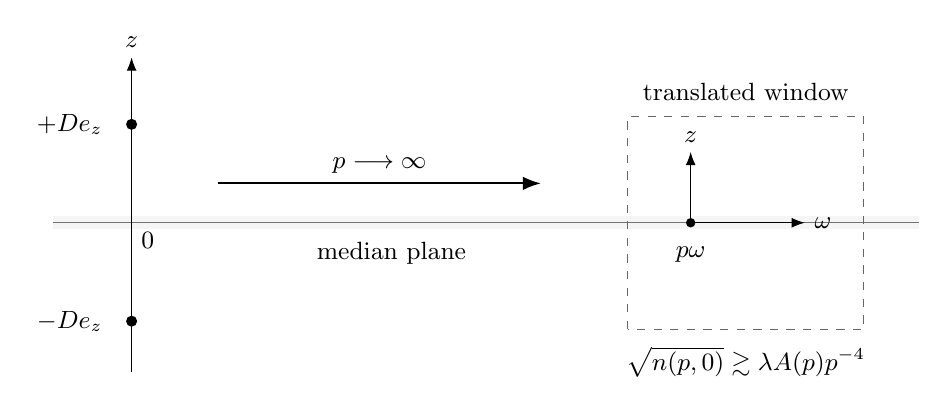
\begin{tikzpicture}[x=1cm,y=1cm,>=Latex,font=\small]
  \fill[black!4] (-1,-0.08) rectangle (10,0.08);
  \draw[black!55] (-1,0) -- (10,0);
  \draw[->] (0,-1.9) -- (0,2.1) node[above] {$z$};
  \fill (0,1.25) circle (2pt) node[left=7pt] {$+De_z$};
  \fill (0,-1.25) circle (2pt) node[left=7pt] {$-De_z$};
  \node[below right] at (0,0) {$0$};
  \node[below] at (3.3,-0.12) {median plane};
  \draw[->,thick] (1.1,0.5) -- (5.2,0.5)
    node[midway,above] {$p\longrightarrow\infty$};
  \draw[dashed,black!60] (6.3,-1.35) rectangle (9.3,1.35);
  \fill (7.1,0) circle (1.7pt) node[below=5pt] {$p\omega$};
  \draw[->] (7.1,0) -- (8.55,0) node[right] {$\omega$};
  \draw[->] (7.1,0) -- (7.1,0.9) node[above] {$z$};
  \node[above] at (7.8,1.43) {translated window};
  \node[below] at (7.8,-1.45) {$\sqrt{n(p,0)}\gtrsim\lambda A(p)p^{-4}$};
\end{tikzpicture}

\caption{A meridional section of the scaled molecule, drawn
schematically and not to scale. The nuclei lie at \(\pm De_z\);
the horizontal line is the median plane \(z=0\). A bounded window
is translated to a distant point \(p\omega\) in that plane.
After normalization by \((A(p)/p)^2\), the limiting density in
the window vanishes quadratically on the plane, although the
actual density there has a smaller nonzero tail. This distinction
drives the limiting-orbital and trace arguments.}
\label{fig:median-plane}
\end{figure}

Trigonometric parametrizations also underlie constrained kinetic-energy
formulations for paired real orbitals~\cite[Section~3.3]{KR25}.
For the Coulomb density \(n\), we minimize
\[
\int_{\R^3}n|\nabla\theta|^2,\qquad
\int_{\R^3}n\sin^2\theta=1,
\]
over odd angles, folded into \([0,\pi/2]\) on the upper half-space.
The orbitals
\[
g=\sqrt n\cos\theta,\qquad h=\sqrt n\sin\theta
\]
have squared norms two and one, respectively. They obey common
formal-potential equations with energies zero and \(d>0\).
A weighted spectral estimate proves that the paired/single
determinant is a kinetic-energy minimum among \emph{all} ensembles
with density \(n\). Consequently, any representing local potential
must agree, up to a constant, with \(V=\Delta g/(2g)\).

If \(V\in\mathcal V\), translations of the orbital equations
force every bounded limiting potential to equal \(d+k^2/2\).
This yields an exterior form bound and hence
\[
e^{ar}g\in H^1(\R^3)
\quad\text{for some }a>k.
\]
The plane trace would then have the same exponential integrability.
But \(\theta=0\) on the plane, so \(g=\sqrt n\) there, and the
nonzero \(\lambda A(r)r^{-4}\) tail makes that trace integral
diverge. This is the contradiction.

Several arguments have uses beyond this example.
Keeping the unperturbed fast channel controls the crossover without
tracking every perturbed excited threshold. Spin orthogonality
prevents cancellation and makes the relevant relative constants
independent of the small level splitting.
The angle construction gives an ensemble kinetic certificate from
a weighted Poincar\'e inequality, even before the formal potential
is known to belong to a standard potential class.
Finally, translated weak potential limits, local form compactness,
and an \(H^1\) trace convert a plane asymptotic into an obstruction
to \(L^{3/2}+L^\infty\), without assuming pointwise convergence of
the potential at infinity. We give the estimates and their
hypotheses explicitly.

\subsection{Organization and conventions}

\Cref{sec:setup} establishes the Coulomb spectral and perturbative
facts. \Cref{sec:channels} proves the uniform density asymptotics
and their fixed-parameter counterpart.
\Cref{sec:angle} constructs the angle and proves the weighted gap.
\Cref{sec:ensemble} establishes the full ensemble certificate and
identifies a hypothetical representing potential.
\Cref{sec:obstruction} proves the fixed-density obstruction
(\Cref{thm:obstruction}) and the qualitative Coulomb family
(\Cref{thm:qualitative-counterexample}).
\Cref{sec:parameters} uses finite sufficient tests to select \(Z\)
and complete \Cref{thm:main}.
\Cref{sec:hxc-first-variation} derives the functional consequence
for the physical density.

All inner products are linear in the second variable.
Norms of ionic channel vectors are Hilbert-space norms.
Spatial reflection means reflection in the median plane; a
simultaneous reflection is applied to all electron coordinates
when discussing a many-electron state. Limits uniform for small
coupling always keep \(D\) fixed first. Later fixed-parameter
limits keep the selected positive coupling fixed.

\section{The Coulomb system and its small-coupling limit}
\label{sec:setup}

Let
\[
 \mathfrak h=L^2(\R^3;\C^2),\qquad
 \mathfrak H_m=\bigwedge\nolimits^m\mathfrak h
\]
be the one-electron and antisymmetric \(m\)-electron spaces.  Spin is
expressed in the basis \(\uparrow,\downarrow\), and spatial reflections
and rotations act trivially on spin.  For \(D>0\), put
\begin{equation}
 u_D(x)=-\frac1{|x-De_z|}-\frac1{|x+De_z|},
 \qquad h_D=-\frac12\Delta+u_D,\qquad e_z=(0,0,1).
 \label{eq:unit-charge-potential}
\end{equation}
The corresponding \(m\)-electron operators are
\begin{equation}
 H_{m,\lambda}
 =\sum_{i=1}^m h_D(x_i)
   +\lambda\sum_{1\le i<j\le m}\frac1{|x_i-x_j|},
 \qquad m=2,3,\quad \lambda\ge0 .
 \label{eq:scaled-coulomb-hamiltonian}
\end{equation}
They act in \(\mathfrak H_m\).  Hardy's inequality in a particle
coordinate, or in a relative coordinate, gives
\[
 \bigl\||x_i-R|^{-1}\psi\bigr\|_2+
 \bigl\||x_i-x_j|^{-1}\psi\bigr\|_2
 \le C\|\nabla\psi\|_2
 \le \varepsilon\|\Delta\psi\|_2+C_\varepsilon\|\psi\|_2 .
\]
Thus these operators are self-adjoint on the antisymmetric part of
\(H^2(\R^{3m};\C^{2^m})\), and their form domain is the corresponding
\(H^1\) space.  The same estimates show that \(\lambda\mapsto
H_{m,\lambda}\) is an analytic family with this common operator domain.
We write \(E_m(\lambda)\) for its ground energy whenever the ground
level under consideration exists.

For a normalized three-electron state, its spin-summed density is
\begin{equation}
 n_\Psi(x)
 =3\sum_{\sigma_1,\sigma_2,\sigma_3}
   \int_{\R^6}
   |\Psi(x,\sigma_1,y_1,\sigma_2,y_2,\sigma_3)|^2\,dy_1\,dy_2 .
 \label{eq:density-definition}
\end{equation}
In particular, \(\int n_\Psi=3\).  Ensemble densities are defined by
linearity, as detailed in \Cref{sec:ensemble}.

\Needspace{5\baselineskip}
\begin{proposition}[Dilation to integer nuclear charges]
\label{prop:scaling}
Suppose that the density of a ground state of \(H_{3,1/Z}\), for a
positive integer \(Z\), has no noninteracting ground-state ensemble
representation with a real spin-independent potential in
\(L^{3/2}(\R^3)+L^\infty(\R^3)\).
The physical Coulomb system with three electrons and charges \(Z,Z\)
at
\[
 (0,0,D/Z),\qquad (0,0,-D/Z)
\]
then has a ground-state density with the same obstruction.
\end{proposition}

\begin{proof}
Use physical coordinates \(\mathbf r_i\) and set \(x_i=Z\mathbf r_i\).
The unitary dilation
\[
 (\mathcal U_Z\psi)(x_1,\ldots,x_m)
 =Z^{-3m/2}\psi(x_1/Z,\ldots,x_m/Z)
\]
leaves spin unchanged.  It transforms the physical Coulomb Hamiltonian
into \(Z^2H_{m,1/Z}\).  In particular, normalizability, the ground-space
property, and antisymmetry are preserved, and
\[
 n_{\rm phys}(\mathbf r)=Z^3 n_{\rm scaled}(Z\mathbf r).
\]
A physical noninteracting representing potential would transform into
\[
 \widetilde v(x)=Z^{-2}v(x/Z).
\]
For a decomposition \(v=v_1+v_\infty\), with
\(v_1\in L^{3/2}\) and \(v_\infty\in L^\infty\), the corresponding
pieces satisfy
\[
 \|Z^{-2}v_1(\,\cdot\,/Z)\|_{3/2}=\|v_1\|_{3/2},
 \qquad
 \|Z^{-2}v_\infty(\,\cdot\,/Z)\|_\infty
 =Z^{-2}\|v_\infty\|_\infty .
\]
The dilation of the representing density matrix preserves its trace
and support in the ground eigenspace.  It would therefore give the
excluded representation of the scaled density.
\end{proof}

\subsection{The two lowest spatial orbitals}

All subsequent one-particle orbitals are spatial orbitals.  For fixed
\(D\) we abbreviate \(u_D\) to \(u\).  Reflection symmetry will mean
reflection in \(z=0\), with \(x=(x_1,x_2,z)\).

\begin{proposition}[Two-centre spectrum]
\label{prop:two-centre-spectrum}
For \(D\ge100\), the two lowest eigenvalues of \(h_D\) are simple.
They have normalized real, axisymmetric eigenfunctions \(b,e\), where
\(b>0\) is even and \(e\) is odd and strictly positive on \(z>0\).
Write
\[
 \epsilon_b=-\frac{\gamma^2}{2},\qquad
 \epsilon_e=-\frac{k_0^2}{2},\qquad
 d_*=\epsilon_e-\epsilon_b .
\]
Then
\begin{equation}
 0<d_*<\frac{100}{D},\qquad
 |\gamma-1|+|k_0-1|<\frac{200}{D}.
 \label{eq:two-centre-numerics}
\end{equation}
The spectrum on \(\{b,e\}^{\perp}\) lies more than \(0.2\) above
\(\epsilon_e\).  In particular, the spectral gap above \(b\) in the
even subspace is greater than \(0.2\).
\end{proposition}

\begin{proof}
Let \(\varphi(x)=\pi^{-1/2}e^{-|x|}\) be the hydrogenic ground state.
We recall the two hydrogenic bounds needed for localization.  After
spherical-harmonic decomposition, the radial operators and first-order
factors are
\[
 H_\ell=-\frac12\frac{d^2}{d\rho^2}
       +\frac{\ell(\ell+1)}{2\rho^2}-\frac1\rho,
 \qquad
 A_\ell=\frac d{d\rho}-\frac{\ell+1}{\rho}+\frac1{\ell+1}.
\]
Here \(H_\ell\) has its Friedrichs realization in
\(L^2((0,\infty),d\rho)\), and \(A_\ell\) is closed from
\(C_c^\infty(0,\infty)\).
On the corresponding Friedrichs form domains, integration by parts gives
\[
 \frac12A_\ell^*A_\ell=H_\ell+\frac1{2(\ell+1)^2},
 \qquad
 \frac12A_\ell A_\ell^*=H_{\ell+1}+\frac1{2(\ell+1)^2}.
\]
The first identity and centrifugal comparison give
\(H_\ell\ge-1/8\) for \(\ell\ge1\).  Also
\(\ker A_0=\operatorname{span}\{\rho e^{-\rho}\}\), and the second
identity gives \(A_0A_0^*\ge3/4\).  The polar decomposition transfers
this last bound to \(A_0^*A_0\) on \((\ker A_0)^\perp\).
Thus the hydrogenic operator has ground energy \(-1/2\) and is
bounded below by \(-1/8\) on \(\varphi^\perp\); the radial
\(\ell=1\) function \(\rho^2e^{-\rho/2}\) attains \(-1/8\).

Choose a Lipschitz angle \(\tau(\rho)\) that is zero for
\(\rho\le D/4\), is \(\pi/2\) for \(\rho\ge D/2\), and is linear
between these radii.  Its slope is \(2\pi/D\).  Around the two nuclei
use cutoffs
\(\chi_\pm(x)=\cos\tau(|x\mp De_z|)\), set equal to zero outside their
respective balls of radius \(D/2\), and complete them by the
nonnegative cutoff \(\chi_{\rm out}\) to a quadratic partition:
\[
 \chi_+^2+\chi_-^2+\chi_{\rm out}^2=1.
\]
The two balls are disjoint.  On either transition annulus the
nonconstant pair is a cosine and a sine, so
\begin{equation}
 \frac12\sum_{\nu\in\{+,-,{\rm out}\}}|\nabla\chi_\nu|^2
 \le \frac{2\pi^2}{D^2}<\frac{20}{D^2}.
 \label{eq:two-centre-ims-cost}
\end{equation}
Lipschitz cutoffs suffice for the form identity; alternatively one may
smooth the ramp with arbitrarily small increases in these constants.

On either inner ball, the attraction of the other nucleus has
magnitude at most \(2/(3D)<1/D\).  On the support of
\(\chi_{\rm out}\), both nuclear distances are at least \(D/4\);
there the total attraction is at most \(8/D\).  Applying the IMS
identity and the hydrogenic ground-energy bound gives
\begin{equation}
 h_D\ge-\frac12-\frac1D-\frac{20}{D^2}
 \quad\text{as a quadratic form}.
 \label{eq:two-centre-bottom-lower}
\end{equation}
Here and below the exterior lower bound \(-8/D\) is larger than the
displayed inner lower bound for \(D\ge100\).

If a test function \(\psi\) is orthogonal to both
\(\chi_\pm\varphi(\,\cdot\,\mp De_z)\), then
\(\chi_\pm\psi\) is orthogonal to the ground state of the corresponding
hydrogenic operator.  The next hydrogenic energy is \(-1/8\).
Consequently,
\begin{equation}
 \langle\psi,h_D\psi\rangle
 \ge\left(-\frac18-\frac1D-\frac{20}{D^2}\right)\|\psi\|_2^2
 \label{eq:two-centre-third-lower}
\end{equation}
on a subspace of codimension two.

For the upper bound, use the two disjointly supported trial functions
\(\chi_\pm\varphi(\,\cdot\,\mp De_z)\).  Their squared norms exceed
\(1/2\), since the hydrogenic mass outside radius \(D/4\) is
\[
 e^{-D/2}\left(1+\frac D2+\frac{D^2}{8}\right)<\frac12.
\]
The ground-state identity for the hydrogenic operator and the bound
\(|\nabla\chi_\pm|\le2\pi/D\) show that their Rayleigh quotients for
\(h_D\) are at most
\begin{equation}
 -\frac12+\frac{4\pi^2}{D^2}
 <-\frac12+\frac{40}{D^2}.
 \label{eq:two-centre-two-upper}
\end{equation}
Their even and odd combinations give the same bound in the two
parity subspaces.  The Coulomb potential is relatively compact with
respect to the free resolvent: one first truncates at infinity and
near the nuclei, and uses local compactness for the bounded remainder.
The omitted nuclear piece has operator norm from \(H^2\) to \(L^2\)
of order \(\sqrt{\varepsilon}\) when cut off to a ball of radius
\(\varepsilon\), by \(H^2\hookrightarrow L^\infty\) and
\(\||x|^{-1}\mathbf 1_{|x|<\varepsilon}\|_2=O(\sqrt\varepsilon)\).
The far-field remainder tends to zero in \(L^\infty\).
Hence the essential spectrum is \([0,\infty)\).
The min--max principle now gives two negative levels, one in each
parity, and no third level below the lower bound in
\Cref{eq:two-centre-third-lower}.

A full-space ground state can be chosen nonnegative by the
absolute-value inequality for its kinetic energy.  It is strictly
positive, including at the nuclei.  One direct way to include those
points is to use
\[
 b=\left(-\frac12\Delta+c\right)^{-1}
       (c+\epsilon_b-u)b,\qquad c>|\epsilon_b|,
\]
whose resolvent kernel is strictly positive; the right-hand side is
nonnegative and nonzero, and \(b\in H^2(\R^3)\) is continuous.
The same argument with the Dirichlet resolvent on \(z>0\) gives
strict positivity of its ground state in that half-space.
Positivity and the usual ground-state simplicity argument identify
the low even level with \(b\) and the low odd level with the odd
extension of that Dirichlet ground state.  Simplicity also follows
from the two-level count above.  The full-space ground state cannot
be odd, so \(\epsilon_b<\epsilon_e\).  Rotation about the \(z\)-axis
preserves the unique normalized positive full-space and half-space
ground states, proving axial symmetry.

Combining \Cref{eq:two-centre-bottom-lower,eq:two-centre-two-upper}
gives
\[
 d_*\le\frac1D+\frac{60}{D^2}<\frac{100}{D}.
\]
The same two bounds place \(\gamma\) and \(k_0\) within
\(200/D\) of \(1\), with the stated bound on their sum.  Finally,
\Cref{eq:two-centre-third-lower,eq:two-centre-two-upper} give the
gap estimate
\[
 \frac38-\frac1D-\frac{60}{D^2}>0.2 .
\]
Since \(e\) is odd, the same lower bound holds above \(b\) in the
even subspace.
\end{proof}

\subsection{Ground states and perturbation}

\begin{proposition}[Small repulsive coupling]
\label{prop:small-coupling}
Fix \(D\ge100\).  For all sufficiently small \(\lambda\ge0\), the
ionic operator \(H_{2,\lambda}\) has a simple isolated ground state,
and \(H_{3,\lambda}\) has a simple isolated ground state
\(\Psi_\lambda\) in the sector \(S_z=1/2\).  Its energy is an absolute
ground energy of \(H_{3,\lambda}\).

The ionic ground state is a spin singlet, is even under simultaneous
reflection of its two spatial coordinates, and is axisymmetric.
The state \(\Psi_\lambda\) is real, axisymmetric, and odd under
simultaneous reflection of its three spatial coordinates.
The states and energies can be chosen analytic near zero; in
particular, their state vectors converge with error \(O(\lambda)\)
in \(H^2\).  At zero coupling,
\begin{equation}
 \Psi_0=b\uparrow\wedge b\downarrow\wedge e\uparrow,\qquad
 E_2(0)=2\epsilon_b,\qquad
 E_3(0)=2\epsilon_b+\epsilon_e .
 \label{eq:zero-coupling-states}
\end{equation}
The ionic state has spatial factor \(b(x_1)b(x_2)\) and the normalized
singlet spin factor.
\end{proposition}

\begin{proof}
At \(\lambda=0\), the Pauli principle fills the spin orbitals in
\Cref{eq:zero-coupling-states}.  In the sector \(S_z=1/2\), moving
the doubly occupied spatial orbital from \(b\) to \(e\) costs
\(d_*>0\); using any further spatial orbital costs a positive gap
by \Cref{prop:two-centre-spectrum}.  The displayed determinant is
therefore a simple isolated ground state in that sector.  The ionic
ground state is likewise simple and isolated.  The noninteracting
ionization thresholds are \(2\epsilon_b\) and \(\epsilon_b\),
respectively, and are strictly above these ground energies.

The common-domain analytic perturbation argument applies to each
isolated rank-one spectral projection; see
\cite[Chapter~VII, \S1.3, Theorem~1.7, and \S2.2, Theorem~2.6]{Kato}.
To include the graph-norm conclusion explicitly, write
\(V_{\rm ee}=\sum_{i<j}|x_i-x_j|^{-1}\) and
\(R_0(\zeta)=(H_{m,0}-\zeta)^{-1}\).  On a contour enclosing only
the relevant zero-coupling level,
\[
 (H_{m,\lambda}-\zeta)^{-1}
 =R_0(\zeta)\bigl(I+\lambda V_{\rm ee}R_0(\zeta)\bigr)^{-1}.
\]
Here \(R_0(\zeta):L^2\to H^2\) and
\(V_{\rm ee}R_0(\zeta):L^2\to L^2\) are bounded uniformly on the
contour.  A Neumann series therefore makes the resolvent analytic
as a map into \(H^2\).  Integrating around the contour, applying the
resulting projection to the unperturbed state, and normalizing gives
a real-analytic state in that space.  Choose its
real phase by positive overlap with the zero-coupling state.
Spectral separation, or the min--max principle with the nonnegative
repulsion, keeps this branch the lowest level of its sector.

It remains to check the absolute three-electron ground property.
In the sectors \(S_z=\pm3/2\), all three spatial orbitals must be
distinct.  Their zero-coupling energy is at least
\(\epsilon_b+\epsilon_e+\epsilon_3\), where
\(\epsilon_3=\inf\sigma(h_D|_{\{b,e\}^\perp})\); it exceeds
\(2\epsilon_b+\epsilon_e\) by more than \(0.2\).
Nonnegative repulsion preserves this lower bound, whereas the
continued \(S_z=1/2\) energy converges to
\(2\epsilon_b+\epsilon_e\).  Spin flip identifies the two
\(S_z=\pm1/2\) ground energies.  These four sectors exhaust the
three-electron spin space, proving the claim.

All the stated symmetries commute with the Hamiltonian and its
spectral projection.  Their eigenvalues at zero coupling persist on
the simple branch.  For axial rotations, one may equivalently note
that the projection of the invariant zero-coupling state is still
invariant.  The ionic singlet subspace is also invariant, so its
spin character persists.
\end{proof}

For the rest of the small-coupling argument define
\begin{equation}
 k=k_\lambda=\sqrt{2\bigl(E_2(\lambda)-E_3(\lambda)\bigr)},\qquad
 A(r)=e^{-kr}r^\beta,\qquad
 \beta=\frac{2-2\lambda}{k}-1 .
 \label{eq:ionization-parameters}
\end{equation}
Thus \(k_\lambda\to k_0\).  Once \(D\) is fixed, the perturbation
interval may be shortened so that
\begin{equation}
 \gamma-k_\lambda\ge\frac12(\gamma-k_0)>0 .
 \label{eq:uniform-fast-slow-separation}
\end{equation}
No lower bound uniform in \(D\) on the length of this interval is
asserted or needed.

\begin{lemma}[Density regularity and compact convergence]
\label{lem:density-regularity}
Regard
\(F_{\rm true}(x)=\sqrt3\,\Psi_\lambda(x,\cdot)\) as a
Hilbert-space-valued function, retaining the removed-electron spin
and all ionic coordinates and spins.  Then
\[
 F_{\rm true}\in H^2(\R^3;\mathcal K),\qquad
 n_\lambda=\|F_{\rm true}\|_{\mathcal K}^2
       \in H^2(\R^3)\cap L^1(\R^3),\qquad
 \sqrt{n_\lambda}\in H^1(\R^3),
\]
where \(\mathcal K\) is the corresponding fiber Hilbert space.
Moreover \(\Delta n_\lambda\in L^1(\R^3)\).
These assertions hold for every \(H^2\) three-electron eigenstate,
with no small-coupling assumption.

For the branch in \Cref{prop:small-coupling},
\(n_\lambda\to n_0=2b^2+e^2\) in \(H^2\) and \(L^1\), hence
uniformly on compact sets; the densities are commonly tight as
\(\lambda\downarrow0\).  Each fixed compact set has a positive
lower bound for \(n_\lambda\) for sufficiently small \(\lambda\).
The density is even and axisymmetric.
\end{lemma}

\begin{proof}
Fubini's theorem applied to the derivatives in the distinguished
coordinate gives the Hilbert-valued \(H^2\) assertion.  In three
dimensions the corresponding Sobolev estimates yield
\[
 \|F_{\rm true}\|_{L^\infty_x(\mathcal K)}
 +\|\nabla_xF_{\rm true}\|_{L^4_x(\mathcal K)}
 \le C\|F_{\rm true}\|_{H^2_x(\mathcal K)} .
\]
The distributional product identities
\begin{align}
 \partial_j n_\lambda
 &=2\operatorname{Re}
      \langle F_{\rm true},\partial_jF_{\rm true}\rangle_{\mathcal K},
 \notag\\
 \partial_i\partial_j n_\lambda
 &=2\operatorname{Re}
      \langle\partial_iF_{\rm true},\partial_jF_{\rm true}\rangle_{\mathcal K}
   +2\operatorname{Re}
      \langle F_{\rm true},\partial_i\partial_jF_{\rm true}\rangle_{\mathcal K}
 \label{eq:density-product-identities}
\end{align}
then prove \(n_\lambda\in H^2\).  The same identities and
Cauchy--Schwarz, now using \(L^2_x\) on both factors, give
\(\Delta n_\lambda\in L^1\).  The norm chain rule gives
\begin{equation}
 \int_{\R^3}|\nabla\sqrt{n_\lambda}|^2
 \le \int_{\R^3}\|\nabla_xF_{\rm true}\|_{\mathcal K}^2 .
 \label{eq:density-kinetic-bound}
\end{equation}

The product estimates also show continuity of
\(F\mapsto\|F\|_{\mathcal K}^2\) from \(H^2_x(\mathcal K)\) to
\(H^2_x\).  Thus the graph-norm convergence in
\Cref{prop:small-coupling} gives the claimed density convergence.
For the \(L^1\) convergence, use
\[
 \|n_\lambda-n_0\|_1
 \le
 \bigl(\|F_{{\rm true},\lambda}\|_2+\|F_{{\rm true},0}\|_2\bigr)
 \|F_{{\rm true},\lambda}-F_{{\rm true},0}\|_2 .
\]
It implies common tightness.  Since \(b\) is continuous and
strictly positive everywhere, \(n_0\ge2b^2\) has a positive minimum
on each compact set.  Uniform convergence gives the corresponding
compact lower bound for \(n_\lambda\).  The spatial symmetries
follow by taking the squared fiber norm.
\end{proof}

The last lemma makes no claim of global positivity from compact
convergence alone.  The exterior argument below supplies positivity
outside a fixed ball uniformly for sufficiently small coupling, and
thereby supplies the global positivity needed for the angle
construction.

\section{Exterior channels and the density near the median plane}
\label{sec:channels}

The leading removal amplitude has a simple zero on the median plane,
but a complementary ionic channel supplies a nonzero density tail
there with the same exponential rate.  This is the nodal-plane
mechanism discussed in \cite[Section~V.A]{GGB}.  We prove the estimates,
including their uniformity as the interaction tends to zero, without
assuming an asymptotic expansion of finitely many Dyson orbitals.

In the perturbative part of this section \(D\) is fixed and sufficiently
large, and \(0\leq\lambda\leq\lambda_D\), where \(\lambda_D>0\) may be
decreased finitely many times.  Exterior radii and constants denoted
by \(C_D\) may depend on \(D\), but not on \(\lambda\) in this interval.
For \(x=(x_1,x_2,z)\), write \(r=|x|\),
\(p=(x_1^2+x_2^2)^{1/2}\), and \(\omega=x/r\) when \(r>0\).
Differentiation in \(p\) keeps \(z\) fixed.  Put
\begin{equation}
 k=\sqrt{2(E_2(\lambda)-E_3(\lambda))},\qquad
 \beta=\frac{2-2\lambda}{k}-1,\qquad A(r)=e^{-kr}r^\beta.
 \label{eq:channel-radial-factor}
\end{equation}
We can arrange that
\begin{equation}
 k>0.99,\qquad \gamma-k\geq\tfrac12(\gamma-k_0)>0.
 \label{eq:channel-rate-separation}
\end{equation}

\begin{proposition}[Density estimates]
\label{prop:density-properties}
For all sufficiently large \(D\) and sufficiently small \(\lambda\geq0\),
the density \(n=n_\lambda\) is positive, even in \(z\), and axisymmetric.
It is smooth away from the nuclei and converges locally uniformly to
\(2b^2+e^2\) as \(\lambda\downarrow0\).

Given \(\eta>0\), first \(D\) can be chosen sufficiently large and then
\(\lambda_D>0\) sufficiently small so that, beyond a radius independent
of \(0\leq\lambda\leq\lambda_D\),
\begin{equation}
 |\partial_r\log n+2k|\leq\eta,\qquad
 \left|\partial_p\log n+2k\frac p r\right|\leq\eta
 \quad(0\leq z\leq p/2).
 \label{eq:density-drift}
\end{equation}
With \(L=10\) and \(m(p,z)=e^{2kp}n(p,z)\), the same choices give
\begin{equation}
 \frac{|m_p|+|m_{pp}|}{m}\leq\eta,\qquad
 \frac{n(p,z_1)}{n(p,z_2)}\leq20
 \quad(0\leq z_1\leq z_2\leq L)
 \label{eq:strip-data}
\end{equation}
for all sufficiently large \(p\), uniformly in that coupling interval.

For each fixed such \(\lambda>0\), there are \(c_\lambda>0\) and
\(P_\lambda<\infty\) such that
\begin{equation}
 \sqrt{n(p,0)}\geq c_\lambda A(p)p^{-4}\qquad(p\geq P_\lambda).
 \label{eq:plane-tail}
\end{equation}
There is a number \(a>0\), depending on \(D,\lambda\), with the following
translation properties.  If \(x_j=p_j\omega_j\) lies in the median plane,
\(p_j\to\infty\), and the horizontal unit vectors \(\omega_j\to\omega_*\),
then
\begin{equation}
 \frac{n(x_j+x)}{(A(p_j)/p_j)^2}
 \longrightarrow a^2z^2e^{-2k\omega_*\cdot x}
 \quad\hbox{locally uniformly for }x=(x_1,x_2,z)\in\R^3.
 \label{eq:plane-translate}
\end{equation}
If \(|x_j|\to\infty\), \(|(x_j)_3|\to\infty\), and
\(x_j/|x_j|\to\omega_*\), then
\begin{equation}
 \frac{n(x_j+x)}{n(x_j)}
 \longrightarrow e^{-2k\omega_*\cdot x}
 \quad\hbox{locally uniformly in }\R^3.
 \label{eq:bulk-translate}
\end{equation}
\end{proposition}

The quantitative uniformity needed for the final parameter prescription
is given in \Cref{eq:quantitative-density-drift} below.  In particular,
the constants remaining after the exterior limit do not involve the
inverse of the small splitting \(d_*\).

\subsection{The fiber equation and an exterior cutoff}

Let \(\cK\) be the Hilbert space of the antisymmetric ionic pair,
including its spin coordinates and the distinguished electron's spin,
restricted to total spin projection \(1/2\).  Regard
\[
 F_{\mathrm{true}}(x)=\sqrt3\,\Psi_\lambda(x,\cdot)
\]
as a \(\cK\)-valued function, with \(\|F_{\mathrm{true}}(x)\|^2=n(x)\).
The ionic operator acts trivially on the distinguished spin.  Set
\[
 B=H_{\mathrm{ion}}-E_2(\lambda),\qquad
 P=|\phi\rangle\langle\phi|,\qquad Q=1-P,\qquad B_Q=B|_{Q\cK},
\]
where \(\phi\) is the normalized ionic singlet tensored with distinguished
spin up.  Only that distinguished spin is compatible with the singlet
and total projection \(1/2\); hence \(P\) has rank one and
\begin{equation}
 B\geq0,\qquad B_Q\geq c_D>0
 \label{eq:ionic-gap}
\end{equation}
uniformly on the small coupling interval.

For normalized spin orbitals \(v,w\), let \(\Phi_{v,w}\) denote their
normalized two-electron determinant.  Expansion of the unperturbed
determinant in the distinguished coordinate gives
\begin{equation}
 \begin{split}
 F_0(x)&=e(x)\phi_0+b(x)G,\\
 \phi_0&=\uparrow\otimes\Phi_{b\uparrow,b\downarrow},\\
 G&=\uparrow\otimes\Phi_{b\downarrow,e\uparrow}
       -\downarrow\otimes\Phi_{b\uparrow,e\uparrow}.
 \end{split}
 \label{eq:unperturbed-fibers}
\end{equation}
Consequently
\begin{equation}
 \|G\|=\sqrt2,\qquad
 \|G_\uparrow\|=\|G_\downarrow\|=1,\qquad B_0G=d_*G.
 \label{eq:core-spin-components}
\end{equation}
The ionic spatial parity of \(G\) is odd, whereas that of \(\phi\) is
even.  Thus \(QG=G\) at every coupling under consideration.

\begin{lemma}[Cutoff channel equation]
\label{lem:channel-cutoff}
There are an exterior \(\cK\)-valued function \(F\), a nonnegative bounded
multiplication operator \(W(x)\) on the ionic variables, and
\(\sigma>\gamma\) such that
\begin{equation}
 \left(-\frac{\Delta_x}{2}+\frac{k^2}{2}+B+u(x)+\lambda W(x)\right)F=R.
 \label{eq:cutoff-channel-equation}
\end{equation}
The operator \(W\) equals \(\sum_{i=1}^2|x-y_i|^{-1}\) for
\(|y|\leq r/2\), vanishes for \(|y|\geq3r/4\), and satisfies
\begin{equation}
 \|\partial_x^\nu W(x)\|_{\cK\to\cK}
 \leq C_\nu r^{-1-|\nu|}.
 \label{eq:cutoff-interaction-symbol}
\end{equation}
Here \(\nu\) is a Cartesian multiindex.  For every fixed integer \(s\),
\begin{equation}
 \|\partial_x^\nu R(x)\|\leq C_{D,s}\lambda e^{-\sigma r}
 \quad(|\nu|\leq s).
 \label{eq:channel-residual}
\end{equation}
Moreover,
\begin{equation}
 \left|\partial_x^\nu\{n(x)-\|F(x)\|^2\}\right|
 \leq C_D e^{-2\sigma r}\quad(|\nu|\leq2),
 \label{eq:density-cutoff-error}
\end{equation}
and \(F-F_0=O(\lambda)\) on each fixed exterior annulus, also in any
fixed finite number of \(x\)-derivatives.
\end{lemma}

\begin{proof}
Put \(\rho=(|x|^2+|y|^2)^{1/2}\).  A configuration-space partition
according to a particle with distance at least a fixed multiple of
\(\rho\) from the origin gives the exterior form bound
\begin{equation}
 H_{3,\lambda}\geq2\epsilon_b-o(1)
 \quad\hbox{on functions supported where }\rho\to\infty.
 \label{eq:configuration-exterior-bound}
\end{equation}
The nuclear attraction of the selected particle is \(O(1/\rho)\);
the other two one-particle operators are each bounded below by
\(\epsilon_b\), and repulsion can be dropped.  The partition has
derivatives \(O(1/\rho)\), so its kinetic localization error tends
to zero.  This argument is uniform for \(0\leq\lambda\leq1\).

The exponent margin needed below already follows for \(D\ge100\)
from \Cref{eq:two-centre-bottom-lower,eq:two-centre-two-upper}:
\[
 \begin{gathered}
 k_0^2\ge1-\frac{80}{D^2},\qquad
 \gamma^2\le1+\frac2D+\frac{40}{D^2},\\
 \frac{10}{9}k_0^2-\gamma^2
 \ge\frac19-\frac2D-\frac{1160}{9D^2}>0.
 \end{gathered}
\]
We can therefore choose
\[
 0<\tau_0<\tau_1<\tau_2<k_0,\qquad \tau_0\sqrt{10/9}>\gamma.
 \]
After decreasing \(\lambda_D\), the exterior bound and
\(E_3(0)=2\epsilon_b-k_0^2/2\) leave a positive margin above the
weight cost \(\tau_2^2/2\).  The exponential-weight identity, first
with an exterior cutoff and a smooth truncated exponent whose
gradient has norm at most one, gives
\begin{equation}
 \|e^{\tau_1\rho}F_{\mathrm{true}}\|_{H^1(\R^9)}
 +\|e^{\tau_1\rho}F_0\|_{H^1(\R^9)}\leq C_D.
 \label{eq:configuration-weight}
\end{equation}
At zero coupling the same argument also gives
\(\|e^{\tau_2\rho}F_0\|_{H^1}\leq C_D\), since \(\tau_2<k_0\).
The finite spin sum is understood.  The estimate also applies to an
inhomogeneous equation: if
\((H_{3,\lambda}-E_3(\lambda))v=f\), then, for a fixed ball \(K\),
\begin{equation}
 \|e^{\tau_1\rho}v\|_{H^1}
 \leq C_D\left(\|e^{\tau_1\rho}f\|_2+\|v\|_{H^1(K)}\right).
 \label{eq:inhomogeneous-weight}
\end{equation}
Indeed the exterior spectral lower bound controls the weighted
\(L^2\) norm by the weight identity and Cauchy--Schwarz.  Combining
a small multiple of the kinetic form estimate with that lower bound
also controls the gradient; the strict margin between \(\tau_1\) and
\(\tau_2\) absorbs its additional weight cost.  Hardy's inequality
absorbs the infinitesimally form-bounded Coulomb terms.  These bounds
are independent of the exponent truncation, which can therefore
be removed.

The equation for \(v=F_{\mathrm{true}}-F_0\) has source
\[
 \bigl(E_3(\lambda)-E_3(0)-\lambda V_{\mathrm{ee}}\bigr)F_0.
 \]
Hardy's inequality, with the spare exponent \(\tau_2\) on \(F_0\),
bounds it by \(C_D\lambda\) in weighted \(L^2\).
The compact term is \(O(\lambda)\) by \Cref{prop:small-coupling}.
Thus
\begin{equation}
 \|e^{\tau_1\rho}(F_{\mathrm{true}}-F_0)\|_{H^1}\leq C_D\lambda.
 \label{eq:weighted-state-difference}
\end{equation}

Choose smooth functions of \(|y|/r\), with values in \([0,1]\), such
that \(\chi=1\) on \(|y|\leq r/3\), \(\chi=0\) on \(|y|\geq r/2\),
and \(\zeta=1\) on \(|y|\leq r/2\), \(\zeta=0\) on
\(|y|\geq3r/4\).  Define
\[
 F=F_0+\chi(F_{\mathrm{true}}-F_0),\qquad
 W=\zeta\sum_{i=1}^2|x-y_i|^{-1}.
 \]
On the support of \(\zeta\), \(|x-y_i|\geq r/4\), proving
\Cref{eq:cutoff-interaction-symbol}.  Denote the operator on the
left of \Cref{eq:cutoff-channel-equation} by \(\mathcal L_\lambda\).
Since \(W\) is exact on the support of \(\chi\),
\begin{equation}
 R=(1-\chi)\mathcal L_\lambda F_0
       +[\mathcal L_\lambda,\chi](F_{\mathrm{true}}-F_0),
 \label{eq:cutoff-residual-identity}
\end{equation}
where
\[
 \mathcal L_\lambda F_0
 =\left\{\lambda\left(|y_1-y_2|^{-1}+W\right)
          -E_3(\lambda)+E_3(0)\right\}F_0.
 \]
Thus every residual term is \(O(\lambda)\) and is supported where
\(|y|\geq r/3\).  There,
\begin{equation}
 \rho\geq\sqrt{10/9}\,r.
 \label{eq:cutoff-geometric-margin}
\end{equation}

We give the derivative details, since higher ordinary derivatives
of the uncut wavefunction across a collision cannot simply be
iterated.  Local \(H^2\) estimates on nested fixed-size configuration
boxes have uniform constants: the Laplacian estimate with cutoffs
and the infinitesimal Coulomb bound absorb the potential terms;
the local energy estimate controls cutoff commutators.  Where
derivatives of \(\chi\) occur, \(x\) is separated from both other
electrons.  Further \(x\)-derivatives of the equation differentiate
only smooth bounded coefficients, while singular ionic coefficients
are independent of \(x\).  Difference quotients followed by these
local estimates give any fixed number of \(x\)-derivatives of the
difference, at size \(O(\lambda)\) in weighted local norms.
In the other residual term, \(F_0\) has the product form
\Cref{eq:unperturbed-fibers}; its \(x\)-derivatives have no
electron-electron singularity, and the ionic Coulomb multiplier
is controlled by Hardy's inequality.  Summing the box estimates
and using Sobolev embedding in the three \(x\)-coordinates gives
\Cref{eq:channel-residual}.  A small loss from \(\tau_1\) toward \(\tau_0\)
absorbs polynomial integration factors.  By
\Cref{eq:cutoff-geometric-margin}, one still has \(\sigma>\gamma\).

Density derivatives in the discarded region require a different
coordinate choice.  Choose smooth pair cutoffs \(\chi_{ij}\in[0,1]\)
equal to one at distances at most \(1\) and zero at distances at least
\(2\), and expand the product of the three identities
\(1=\chi_{ij}+(1-\chi_{ij})\).
For each term use the connected components of its near-edge graph
as clusters.  They have diameter at most \(4\), and distinct clusters
are separated by at least \(1\).  Nested boxes in which each
particle moves by less than \(1/8\) preserve a positive separation.
The cluster containing \(x\) is far from the nuclei when \(r\) is large.
Translate with \(x\) all other
variables in that cluster.  A derivative in the translated
\(x\)-coordinate is the sum of the corresponding particle
derivatives.  It annihilates within-cluster Coulomb singularities
and singularities involving only outside particles; every
coefficient differentiated is smooth with uniformly bounded
derivatives.  Nested-box energy and elliptic estimates can
therefore be iterated in these three translation directions.
This is the parallel-derivative method of
\cite[preprint version, Proposition~1.10 and Section~6]{FS18}; here the fixed
separations make the constants uniform, while
\Cref{eq:configuration-weight,eq:weighted-state-difference}
preserve the requisite exponential weights.

The difference \(n-\|F\|^2\) is a sum of integrals of products of
\(F_{\mathrm{true}}\) and \(F_0\), with coefficients supported where
\(|y|\geq r/3\).  After the coordinate changes just described,
differentiate these integrals and apply Cauchy--Schwarz to the
weighted local estimates.  Each product has two exponentially
decaying factors.  Sobolev embedding in the three translation
directions and \Cref{eq:cutoff-geometric-margin} give
\Cref{eq:density-cutoff-error}, after another arbitrarily small
loss of exponent.  To obtain smoothness on a compact set disjoint from
the nuclei, replace the pair-cutoff radii \(1,2\) by
\(\varepsilon,2\varepsilon\), with \(\varepsilon\) smaller than one
sixteenth of the set's distance from the nuclei.  The cluster containing
\(x\) has diameter at most \(4\varepsilon\); sufficiently small nested
boxes therefore keep it away from the nuclei and preserve the
intercluster separation.  The same argument without discarding a tail
then proves smoothness of the density there.
On fixed exterior annuli the differentiated local estimates also
give the claimed \(O(\lambda)\) convergence of \(F-F_0\).
\end{proof}

\subsection{Localized multipoles and the slow channel}

Reduced ionic inverses preserve the moment bounds needed below.
Let \(\rho_y=(1+|y|^2)^{1/2}\).  For some \(s_D>0\),
\(\phi\) is bounded uniformly in \(e^{s_D\rho_y}H^2_y\).
Moreover, if \(e^{s\rho_y}v\in L^2\), then
\begin{equation}
 e^{s'\rho_y}B_Q^{-1}Qv\in H^2_y
 \quad\hbox{for some }0<s'<s,
 \label{eq:weighted-ionic-inverse}
\end{equation}
with uniform bounds on the small coupling interval.
To justify this, conjugate the ionic operator by a small exponential
with smooth truncated exponent.  The added first-order term has
small relative operator bound and the added zeroth-order term is
bounded and small.  An isolated contour around the ground
eigenvalue has uniformly bounded conjugated resolvents.  Applying
the resulting projection to a compactly supported vector with
nonzero ground-state overlap proves localization of \(\phi\).
The operator \(B+P\) has a bounded inverse into \(H^2_y\).
Its conjugated finite-rank term is now bounded by the localization
of \(\phi\), so the same inverse perturbation argument applies.
Restriction to \(Q\) proves \Cref{eq:weighted-ionic-inverse}.
Bounds are independent of the exponent truncation.  Polynomial
multiplication is harmless after decreasing the exponent again;
only finitely many such decreases will be used.

On these localized vectors, finite Taylor expansion gives
\begin{equation}
 W=\frac2r+\frac{W_2(\omega)}{r^2}
       +\frac{W_3(\omega)}{r^3}+\cdots,\qquad
 W_2(\omega)=\omega\cdot(y_1+y_2).
 \label{eq:ionic-multipoles}
\end{equation}
An expansion through \(r^{-m}\), applied to a vector bounded in
one of the preceding weighted spaces, has remainder \(O(r^{-m-1})\),
with Cartesian derivative of order \(|\nu|\) bounded by
\(O(r^{-m-1-|\nu|})\).
On \(|y|\leq3r/4\), the Taylor remainder is bounded by a constant
times \(|y|^m r^{-m-1}\).  Outside this region the polynomial
moments of the localized vector bound the omitted cutoff tail
exponentially.  Differentiation gives the same symbol bounds.
These are expansions on localized vectors, not operator-norm
expansions on all of \(\cK\).  Similarly write
\[
 u=-2/r+\sum_{j\geq2}U_j(\omega)r^{-j},\qquad
 U_2=0,\qquad U_3=-D^2(3\omega_z^2-1),
 \]
with finite-order Taylor remainders understood.

\begin{lemma}[Slow-channel expansion]
\label{lem:channel-expansion}
Write \(PF=\phi f\).  With every fixed finite number of angular
derivatives,
\begin{equation}
 \|F\|=O(A),\qquad \|QF\|=O(A/r^2).
 \label{eq:channel-leading-bounds}
\end{equation}
There are smooth real odd scalar functions \(a_0,a_1,a_2\) on
\(\mathbb S^2\) such that
\begin{equation}
 f=A\left(a_0+\frac{a_1}{r}+\frac{a_2}{r^2}+\mathcal E\right).
 \label{eq:projected-channel-expansion}
\end{equation}
For each fixed angular differential operator \(\Omega^\ell\),
\begin{equation}
 \Omega^\ell\mathcal E=O(r^{-3}),\qquad
 \partial_r\Omega^\ell\mathcal E=O(r^{-4}),\qquad
 \partial_r^2\Omega^\ell\mathcal E=O(r^{-4}).
 \label{eq:scalar-remainder-derivatives}
\end{equation}
The radial remainders are odd in \(\omega_z\); in particular their
bounds without angular differentiation gain a factor
\(|\omega_z|\), also after one or two radial derivatives.
All bounds are uniform for small \(\lambda\).
Furthermore \(a_0^\lambda\to a_0^0\) in \(C^1(\mathbb S^2)\), and
phases can be chosen so that
\begin{equation}
 \inf_{\omega_z>0}\frac{a_0^\lambda(\omega)}{\omega_z}>c_D>0.
 \label{eq:simple-angular-zero}
\end{equation}
Finally,
\begin{equation}
 b=e^{-\gamma r}r^{2/\gamma-1}
       \bigl(b_\infty(\omega)+O(r^{-1})\bigr),\qquad
 \min_{\mathbb S^2}b_\infty>0,
 \label{eq:fast-orbital-expansion}
\end{equation}
with angular derivatives and two radial derivatives of the expansion.
\end{lemma}

\begin{proof}
The ionic gap and multipole estimate imply
\[
 PW\phi=(2/r+O(r^{-2}))\phi,\qquad QW\phi=O(r^{-2}).
 \]
Splitting a vector into \(P+Q\) and applying Young's inequality to
the off-diagonal term, while retaining half the positive \(Q\)-gap,
gives
\begin{equation}
 B+\lambda W\geq 2\lambda/r-C_D/r^2.
 \label{eq:ionic-schur-bound}
\end{equation}
The norm \(N(x)=\|F(x)\|\) consequently satisfies
\[
 \left(-\Delta_x/2+k^2/2-(2-2\lambda)/r-C_D/r^2\right)N\leq\|R\|.
 \]
Take the real inner product of the vector equation with \(F/\|F\|\)
and use \(|\nabla\|F\||\leq\|\nabla F\|\).  Replacing the norm by
\((\|F\|^2+\varepsilon^2)^{1/2}\) proves the weak inequality also
at zeros.  The unbounded ionic operator is handled through its
quadratic form, or by bounded spectral truncations.

Applying this scalar operator to \(A(1-M/r)\), and dividing by \(A\),
gives \(r^{-2}\) coefficient
\[
 kM-\beta(\beta+1)/2-C_D.
 \]
Choose \(M\) to make this positive, and start outside \(r>2M\).
A sufficiently large multiple dominates the inner boundary value
and the exponentially smaller source, yielding \(N=O(A)\) by
exterior comparison.  The latter can be proved by testing the
positive part of the difference with cutoffs: the zeroth-order
coefficient is positive sufficiently far out, both functions
decay, and the cutoff error tends to zero.
The \(Q\)-equation has source
\(-\lambda QW\phi f+QR=O(A/r^2)\).  Its norm inequality retains
the positive constant \(c_D\) in addition to \(k^2/2+u\), so
\(A/r^2\) is a supersolution at sufficiently large radius.  This
proves \Cref{eq:channel-leading-bounds}.

Rotation fields \(\Omega\) acting on \(x\) commute with
\(\Delta_x,B,P,Q\).  Although \(\|\Omega^jW\|=O(r^{-1})\),
one has \(\|\Omega^jW\phi\|=O(r^{-2})\) for \(j\geq1\), and
\(\Omega^ju=O_D(r^{-3})\).
Suppose the two leading bounds hold for fewer than \(s\) rotations.
Every commutator source for \(\Omega^sF\) is \(O(A/r^2)\):
its \(P\)-part uses the improved estimate on \(W\phi\), and its
\(Q\)-part uses \(O(r^{-1})O(A/r^2)\).
First the full norm comparison gives \(\Omega^sF=O(A)\);
then the \(Q\)-equation and its gap give \(Q\Omega^sF=O(A/r^2)\).
This closes the induction.  The absolute decay needed for
comparison follows from the cutoff construction, allowing a small
exponential loss for the polynomial coefficients of rotation fields.

Set \(h_0=f/A\), and define
\begin{equation}
 K_j=-\tfrac12\Delta_{\mathbb S^2}
       -\tfrac12(\beta-j)(\beta-j+1),\qquad
 c_m=U_m+\lambda\langle\phi,W_m\phi\rangle.
 \label{eq:angular-recursion-operators}
\end{equation}
Axial symmetry and reflection give \(c_2=0\).
The projected equation conjugated by \(A\) is
\begin{equation}
 -\tfrac12h_0''+
 \left(k-\frac{\beta+1}{r}\right)h_0'
 +\frac{K_0+c_2}{r^2}h_0+\frac{c_3}{r^3}h_0+\cdots
 =O(r^{-4}),
 \label{eq:projected-radial-equation}
\end{equation}
with any fixed number of angular derivatives.
The off-diagonal source has this order because
\(\|PWQ\|=\|QW\phi\|=O(r^{-2})\) and \(QF=O(A/r^2)\).

For the radial step, if a bounded angular-valued function \(H\)
satisfies
\[
 -\tfrac12H''+\left(k-\frac{\beta+1}{r}\right)H'=G(r),
 \qquad G(r)=O(r^{-q}),\quad q>1,
 \]
then
\begin{equation}
 H'(r)=2e^{2kr}r^{-2(\beta+1)}
       \int_r^\infty e^{-2ks}s^{2(\beta+1)}G(s)\,ds.
 \label{eq:radial-integrating-factor}
\end{equation}
The other homogeneous branch grows exponentially and is excluded
by boundedness.  The integral is \(O(r^{-q})\), uniformly for the
present bounded \(\beta\) and positive lower bound on \(k\);
thus \(H\) has a limit with error \(O(r^{1-q})\).
Initially the right side of the radial equation is \(O(r^{-2})\),
since all needed angular derivatives of \(h_0\) are bounded.
Hence \(h_0\to a_0\), with error \(O(r^{-1})\).
Set
\begin{equation}
 a_1=\frac{(K_0+c_2)a_0}{k},\qquad
 a_2=\frac{(K_1+c_2)a_1+c_3a_0}{2k}.
 \label{eq:scalar-channel-recursion}
\end{equation}
Subtracting \(a_0+a_1/r\) cancels order two; the integrating factor
improves the remainder to \(O(r^{-2})\), with derivative
\(O(r^{-3})\).  Subtracting \(a_2/r^2\) cancels order three,
giving \(\mathcal E=O(r^{-3})\) and \(\mathcal E'=O(r^{-4})\).
The equation gives \(\mathcal E''=O(r^{-4})\).
The same argument with finitely more angular derivatives at each
step proves \Cref{eq:scalar-remainder-derivatives}.
Reflection makes \(f,a_j\), and all radial remainders odd.
The mean-value theorem in the transverse angular coordinate gives
the additional factor at the equator.

On a fixed radius, the projected function and its angular derivatives
converge by the local estimates in \Cref{lem:channel-cutoff}.
Since \(\|f/A-a_0\|_{C^1}\leq C_D/r\) uniformly, first choosing
the radius large and then sending \(\lambda\) to zero proves
\(C^1\) convergence of \(a_0^\lambda\).
At zero coupling the scalar equation for \(e\) on the upper half-space
has a subsolution which is a positive multiple of
\[
 e^{-k_0r}r^{2/k_0-1}\omega_z(1+M/r).
 \]
After division by the radial factor and \(\omega_z\), the controlling
\(r^{-2}\) coefficient contains \(-k_0M\); it dominates the bounded
angular and scalar corrections for large \(M\).
Positivity of \(e\) on an inner hemisphere and the boundary point
lemma on its equator supply a strictly positive starting multiple,
including the equatorial limit.  Exterior comparison proves
\(\inf a_0^0/\omega_z>0\).  Oddness and \(C^1\) convergence give
\Cref{eq:simple-angular-zero}.  The identical scalar argument for
\(b\), without an angular zero and with rate \(\gamma\), proves
\Cref{eq:fast-orbital-expansion}; positivity on the compact inner
sphere gives \(\min b_\infty>0\).
\end{proof}

\subsection{The first nonzero complementary term on the plane}

The scalar channel's oddness forces it to vanish on the median plane.
We now identify the complementary term that supplies its missing
density there, and control its error before comparing it with the
retained fast term \(bG\).

\begin{lemma}[Complementary expansion and plane coefficient]
\label{lem:plane-coefficient}
There are smooth exponentially localized \(Q\cK\)-valued angular
coefficients \(T_2,T_3,T_4\), bounded uniformly for small \(\lambda\),
such that
\begin{equation}
 QF=bG+\lambda A
       \left(\frac{T_2}{r^2}+\frac{T_3}{r^3}+\frac{T_4}{r^4}\right)
       +\mathcal E_Q,\qquad
 \|\partial_x^\nu\mathcal E_Q\|
       \leq C_D\lambda Ar^{-5}\quad(|\nu|\leq2).
 \label{eq:complementary-expansion}
\end{equation}
Writing \(Y_z=y_{1z}+y_{2z}\), one has
\begin{equation}
 \begin{split}
 T_2&=-a_0B_Q^{-1}QW_2\phi,\\
 T_2|_{\omega_z=0}&=T_3|_{\omega_z=0}=0,\\
 T_4|_{\omega_z=0}
   &=\frac12B_Q^{-1}\Delta_{\mathbb S^2}T_2|_{\omega_z=0}
     =-a_0'(0)B_Q^{-2}QY_z\phi .
 \end{split}
 \label{eq:equatorial-coefficient}
\end{equation}
The last vector has norm bounded below by a positive constant at
fixed \(D\), uniformly for sufficiently small \(\lambda\).
All \(T_j\) have distinguished spin up.
\end{lemma}

\begin{proof}
On localized angular coefficients define
\[
 C_m=U_m\,\mathrm{id}_{Q\cK}+\lambda QW_mQ.
 \]
The qualification is essential: \(W_m\), and hence \(C_m\), can
be unbounded on arbitrary ionic vectors.  Their action on the
localized vectors in this proof is controlled by
\Cref{eq:weighted-ionic-inverse,eq:ionic-multipoles}.
On a term \(r^{-j}T(\omega)\), the conjugated \(Q\)-operator has
expansion
\begin{equation}
 r^{-j}B_QT-jk r^{-j-1}T
 +r^{-j-2}K_jT+\sum_{m\geq2}r^{-j-m}C_mT.
 \label{eq:complementary-recursion-action}
\end{equation}
The source from \(P\), after division by \(\lambda A\), is
\(-QW\phi\,f/A\).  Its coefficients of orders two through four are
\[
 \begin{split}
 S_2&=-a_0QW_2\phi,\\
 S_3&=-a_1QW_2\phi-a_0QW_3\phi,\\
 S_4&=-a_2QW_2\phi-a_1QW_3\phi-a_0QW_4\phi.
 \end{split}
 \]
We therefore define the coefficients by
\begin{equation}
 \begin{split}
 B_QT_2&=S_2,\\
 B_QT_3&=S_3+2kT_2,\\
 B_QT_4&=S_4+3kT_3-(K_2+C_2)T_2.
 \end{split}
 \label{eq:complementary-recursion}
\end{equation}
Repeated use of \Cref{eq:weighted-ionic-inverse}, decreasing a
positive weight after polynomial multiplication when necessary,
gives smooth localized coefficients with every finite angular
derivative bound used here.  The nuclear quadrupole has already
entered \(a_2\) in \Cref{eq:scalar-channel-recursion};
the operator \(C_3\) acts directly on this complementary expansion
first at order five.

Every \(S_j\) vanishes on the equator because its scalar factors
\(a_i\) are odd.  The first two recursion equations give
\(T_2=T_3=0\) there.  In the third equation all terms except the
angular Laplacian of \(T_2\) also vanish.  At the equator
\(a_0=\Delta_{\mathbb S^2}a_0=0\), while
\[
 \nabla_{\mathbb S^2}a_0=a_0'(0)e_z,\qquad
 \partial_{\omega_z}W_2=Y_z.
 \]
The product rule in \(T_2=-a_0B_Q^{-1}QW_2\phi\) proves
\Cref{eq:equatorial-coefficient}, with its stated sign and factor.
The slope is nonzero by \Cref{eq:simple-angular-zero}.
Moreover \(Y_z\phi\) is ionic-odd, so \(QY_z\phi=Y_z\phi\).
This vector cannot vanish: the zero set of the multiplier \(Y_z\)
is a measure-zero hyperplane, which cannot support a nonzero
\(L^2\) vector.  Injectivity of \(B_Q^{-2}\) proves nonvanishing.
Continuity of the localized resolvents and vectors gives the
uniform lower bound for small \(\lambda\).  All operators in the
recursion preserve the distinguished spin, so each \(T_j\) has
spin up.

We next prove the remainder with its asserted uniformity.
The retained vector \(bG\) solves the homogeneous \(Q\)-equation
at \(\lambda=0\).  Since \(QG=G\), its perturbed residual is
\begin{equation}
 \begin{split}
 \mathcal L_{\lambda,Q}(bG)
 &=bQ\left\{\lambda\left(|y_1-y_2|^{-1}+W\right)
                 -E_3(\lambda)+E_3(0)\right\}G\\
 &=O(\lambda b),
 \end{split}
 \label{eq:fast-channel-residual}
\end{equation}
also through two ordinary \(x\)-derivatives.
Hardy's inequality controls the ionic Coulomb factor on \(G\);
the other \(x\)-dependent factors are smooth in the exterior.
By \Cref{eq:channel-rate-separation,eq:fast-orbital-expansion},
\begin{equation}
 b/A\leq C_D e^{-(\gamma-k_0)r/2}r^{C_D}.
 \label{eq:fast-term-absorption}
\end{equation}
Thus the residual is bounded by \(C_D\lambda Ar^{-5}\), uniformly
in \(\lambda\).  No equality of perturbed and unperturbed excited
thresholds is being assumed.

The matched slow terms have residual \(O(\lambda Ar^{-5})\).
The same bound holds through two Cartesian derivatives:
finite multipole remainders have symbol bounds on the localized
coefficients, and the scalar remainder is multiplied by
\(\lambda QW\phi=O(\lambda r^{-2})\).
The three bounds in \Cref{eq:scalar-remainder-derivatives} suffice;
one does not need the stronger assertion
\(\partial_r^2\mathcal E=O(r^{-5})\).
The source \(QR\) is exponentially smaller.
Hence \(\mathcal E_Q\) satisfies a \(Q\)-equation with a source
of this size, including two derivatives.  On a fixed large
starting sphere its value is \(O(\lambda)\), since \(QF=bG\)
at zero coupling and all fixed-radius data converge at that rate.
The positive \(Q\)-gap makes a sufficiently large multiple of
\(\lambda Ar^{-5}\) a scalar norm supersolution which dominates
both the source and boundary value.  Exterior comparison gives
the undifferentiated remainder bound.

For the derivative upgrade it is important to include the unbounded
ionic operator.  For compactly supported \(v\) with values in
\(\operatorname{Dom}B_Q\), Fourier transform in \(x\) and the
spectral resolution of \(B_Q\geq0\) give
\begin{equation}
 \|D_x^2v\|_2+\|B_Qv\|_2
 \leq C\|(-\Delta_x/2+B_Q)v\|_2.
 \label{eq:positive-ionic-elliptic-estimate}
\end{equation}
Indeed \(|\xi|^2\) and a spectral value \(b\geq0\) are each bounded
by a fixed multiple of \(|\xi|^2/2+b\).
For the local estimate, first control \(\nabla_xv\) by the
cutoff energy identity and then apply
\Cref{eq:positive-ionic-elliptic-estimate} with a second cutoff.
The remaining coefficient \(k^2/2+u+\lambda QWQ\) and its
\(x\)-derivatives are bounded operators on exterior unit balls,
uniformly in their centers.  Since \(B_Q\) is independent of \(x\),
difference quotients and two further local estimates give
\[
 \|\mathcal E_Q\|_{H_x^4(B(x,1/2);\cK)}
 \leq C_D\lambda A(r)r^{-5}.
 \]
The source derivatives and the already proved pointwise bound
control the right side on a larger ball; \(A\) varies by a bounded
factor there.  Hilbert-valued Sobolev embedding in dimension three,
\(H^4\hookrightarrow C^{2,\alpha}\) for \(\alpha<1/2\), gives
the two pointwise derivative bounds in
\Cref{eq:complementary-expansion}.
\end{proof}

\subsection{Uniform comparison of the three density scales}

The coefficient calculation concerns the eventual tail at a fixed
positive coupling.  To obtain a common exterior radius as the coupling
tends to zero, we must also control the region where the fast term and
the induced plane term are comparable.  Keeping all three scales in
the following lower bound makes that comparison uniform.

\begin{proof}[Proof of \Cref{prop:density-properties}]
Put \(t=\omega_z\) and
\[
 T_{\mathrm{eq}}=T_4|_{t=0},\qquad
 M(x)=\phi f(x)+b(x)G+\lambda A(r)r^{-4}T_{\mathrm{eq}}.
 \]
Axial symmetry and \Cref{eq:equatorial-coefficient} make
\(T_{\mathrm{eq}}\) independent of equatorial azimuth.
Smoothness and the zeros of \(T_2,T_3\) give
\[
 \|T_2(\omega)\|+\|T_3(\omega)\|
       +\|T_4(\omega)-T_{\mathrm{eq}}\|\leq C_D|t|.
 \]
The estimate holds on the whole sphere by compactness away from
the equator.  For any distinguished-spin-up \(Q\)-vector \(S\),
\Cref{eq:core-spin-components} implies
\[
 |\langle bG,S\rangle|
 \leq |b|\,\|S\|=2^{-1/2}\|bG\|\,\|S\|.
 \]
Therefore
\begin{equation}
 \begin{split}
 (1-2^{-1/2})(2b^2+\|S\|^2)
 &\leq\|bG+S\|^2\\
 &\leq(1+2^{-1/2})(2b^2+\|S\|^2).
 \end{split}
 \label{eq:spin-noncancellation}
\end{equation}
The \(P\)-component is orthogonal to both these terms.  The simple
angular zero and positive lower bound on \(\|T_{\mathrm{eq}}\|\)
give
\[
 \|M\|\geq c_D(A|t|+b+\lambda Ar^{-4}).
 \]
The complementary expansion gives
\[
 \|F-M\|\leq C_D\lambda A(r^{-2}|t|+r^{-5})=o_D(\|M\|),
 \]
uniformly in small \(\lambda\) as the radius increases.
Consequently
\begin{equation}
 \|F\|\geq c_D(A|\omega_z|+b+\lambda Ar^{-4}).
 \label{eq:three-scale-lower-bound}
\end{equation}
In addition, there is the absolute bound
\begin{equation}
 b/\|F\|\leq2.
 \label{eq:absolute-core-ratio}
\end{equation}
The distinguished-down-spin component of \(M\) has norm \(b\).
Increase the radius so that \(\|F-M\|\leq\|M\|/2\); then
\[
 \|F\|\geq\|M\|-\|F-M\|\geq\|M\|/2\geq b/2.
\]
Only the radius, not the constant \(2\),
depends on \(D\).
The cutoff errors are relatively negligible because
\[
 e^{-2\sigma r}/b^2\longrightarrow0\qquad(\sigma>\gamma).
 \]
This proves exterior positivity of \(n\); positivity on the
remaining compact set follows from
\Cref{lem:density-regularity} after decreasing \(\lambda_D\).
Symmetry, compact convergence, and exterior smoothness have
already been proved.

We verify differentiated comparisons through the moving crossover.
The projected remainders and their first two radial derivatives
are odd, so their angular derivative bounds supply the factor
\(|t|\).  Their errors can thus be divided by the first lower
scale in \Cref{eq:three-scale-lower-bound}.
For the complementary error,
\[
 \frac{\|\partial_x^\nu\mathcal E_Q\|}{\|F\|}
 \leq C_D/r\quad(|\nu|\leq2,\ \lambda>0),
 \]
using the third lower scale.  At \(\lambda=0\) this error is zero.
Differentiating the explicit slow terms with \(\partial_r+k\)
leaves only inverse powers of \(r\).
For the fast orbital,
\[
 (\partial_r+k)b=(k-\gamma)b+O_D(b/r),\qquad
 (\partial_r+k)^2b=(k-\gamma)^2b+O_D(b/r).
 \]
It follows, with \(\delta_\lambda=k-\gamma\), that
\begin{equation}
 \begin{split}
 (\partial_r+k)F&=\delta_\lambda bG+o_D(\|F\|),\\
 (\partial_r+k)^2F&=\delta_\lambda^2bG+o_D(\|F\|),
 \end{split}
 \label{eq:radial-relative-derivatives}
\end{equation}
where the ratios denoted by \(o_D(1)\) tend to zero uniformly
in the chosen coupling interval.

At fixed \(z\), \(\partial_p\) has radial part
\((p/r)\partial_r\) and angular part of size \(O(|t|/r)\)
on \(0\leq z\leq p/2\).
Applying it once or twice to smooth odd angular coefficients
retains a factor \(|t|\), together with the corresponding
inverse powers of \(r\).  Thus
\[
 \left(\partial_p+k\frac p r\right)F
 =\delta_\lambda\frac p r\,bG+o_D(\|F\|).
 \]
On \(0\leq z\leq L\), \(1-p/r=O_L(p^{-2})\) is negligible.
With \(D_p=\partial_p+k\),
\begin{equation}
 D_pF=\delta_\lambda bG+o_D(\|F\|),\qquad
 D_p^2F=\delta_\lambda^2bG+o_D(\|F\|).
 \label{eq:horizontal-relative-derivatives}
\end{equation}
These estimates include angular derivatives of the displayed
\(T_j\): their zeros are retained for \(T_2,T_3\), whereas the
extra angular factor for \(T_4\) is bounded using the first lower
scale.  The ordinary derivative bounds handle \(\mathcal E_Q\)
directly.

By \Cref{eq:absolute-core-ratio}, \(\|bG\|/\|F\|\leq2\sqrt2\).
The identity
\[
 (\partial_r+2k)\|F\|^2
 =2\operatorname{Re}\langle F,(\partial_r+k)F\rangle
 \]
and its horizontal version bound the normalized first derivatives
by \(4\sqrt2|\delta_\lambda|+o_D(1)\).
Also
\[
 (\partial_p+2k)^2\|F\|^2
 =2\|D_pF\|^2+
  2\operatorname{Re}\langle F,D_p^2F\rangle
 \]
gives the normalized second-derivative bound
\((16+4\sqrt2)\delta_\lambda^2+o_D(1)\) in the strip.
The differentiated cutoff errors remain relatively negligible.
In particular, there is \(\rho_D(R)\downarrow0\), independent
of small \(\lambda\), such that
\begin{equation}
 \begin{split}
 \max\Bigg\{&
 \sup_{r\geq R}|\partial_r\log n+2k|,\ 
 \sup_{\substack{r\geq R\\0\leq z\leq p/2}}
       \left|\partial_p\log n+2k\frac p r\right|,\\
 &\sup_{\substack{p\geq R\\0\leq z\leq L}}
       \frac{|m_p|+|m_{pp}|}{m}\Bigg\}
 \leq100(|\gamma-k|+|\gamma-k|^2)+\rho_D(R).
 \end{split}
 \label{eq:quantitative-density-drift}
\end{equation}
All \(D\)-dependent coefficients other than the fast exponential
rate have entered the vanishing function \(\rho_D\).
Since \(\gamma-k_0\to0\) as \(D\to\infty\) and \(k\to k_0\)
as \(\lambda\downarrow0\), this proves the derivative assertions
in \Cref{eq:density-drift,eq:strip-data}.

For the vertical ratio the expansions give, uniformly on
\(0\leq z\leq L\),
\begin{equation}
 \begin{split}
 F(p,z)={}&\phi a_0'(0)A(p)z/p+b(p,0)G
               +\lambda A(p)p^{-4}T_{\mathrm{eq}}\\
 &+o_D\bigl(A(p)z/p+b(p,0)+\lambda A(p)p^{-4}\bigr).
 \end{split}
 \label{eq:strip-comparison-vector}
\end{equation}
The last coefficient tends to zero uniformly in \(\lambda,z\),
and the error is relatively small compared with the norm of
the three-term comparison vector by
\Cref{eq:spin-noncancellation}.
Indeed \(r-p=O_L(p^{-1})\); after including the lower radial terms,
the projected factor is \(a_0'(0)z/p+O_D(z/p^2)\);
and \(b(p,z)/b(p,0)=1+O_D(p^{-1})\).
The \(T_2,T_3\) terms are \(O_D(\lambda A z/p^3)\);
all other errors have the displayed bound by
\Cref{eq:three-scale-lower-bound}.
The squared comparison norm lies between \(1-1/\sqrt2\) and
\(1+1/\sqrt2\) times
\[
 |a_0'(0)|^2A(p)^2z^2/p^2+
 2b(p,0)^2+\lambda^2A(p)^2p^{-8}\|T_{\mathrm{eq}}\|^2.
 \]
This expression is nondecreasing in \(z\).
The ratio of the constants is \(3+2\sqrt2<6\);
after absorbing uniformly small errors, the ratio in
\Cref{eq:strip-data} is at most \(20\).

Now fix \(\lambda>0\).  On the plane \(f=0\) and \(T_2=T_3=0\).
Since \(b=o(Ap^{-4})\), the complementary expansion yields
\[
 F(p,0)=\lambda A(p)p^{-4}T_{\mathrm{eq}}+o(A(p)p^{-4}).
 \]
The coefficient is nonzero and the density cutoff error is
exponentially smaller, proving \Cref{eq:plane-tail}.

For plane-centered \(x_j=p_j\omega_j\), put \(r_j(x)=|x_j+x|\).
Uniformly on compact displacement sets,
\[
 r_j(x)-p_j\to\omega_*\cdot x,\qquad
 p_jz/r_j(x)\to z,\qquad
 A(r_j(x))/A(p_j)\to e^{-k\omega_*\cdot x}.
 \]
The projected expansion and its simple angular zero imply
\[
 \frac{PF(x_j+x)}{A(p_j)/p_j}
 \longrightarrow\phi a_0'(0)z e^{-k\omega_*\cdot x}.
 \]
The complementary part divided by this normalization tends
uniformly to zero.  Its fast term is exponentially smaller;
the \(T_2,T_3\) terms retain the angular zero and the plane
term is \(O(Ap_j^{-4})\).
The cutoff error is negligible.  Squaring gives
\Cref{eq:plane-translate} with \(a=|a_0'(0)|>0\).

Finally suppose \(r_j=|x_j|\to\infty\) and \(|z_j|\to\infty\).
Reflection reduces the proof to \(z_j>0\).
If \(\omega_{j,z}\) stays bounded below, the conclusion follows
directly from the smooth nonzero projected angular coefficient.
Otherwise \(t_j=z_j/r_j\to0\), and
\[
 \frac{b(r_j)}{A(r_j)t_j}\to0,\qquad
 \frac{\lambda A(r_j)r_j^{-4}}{A(r_j)t_j}
       =\frac{\lambda}{r_j^3z_j}\to0.
 \]
The \(T_2,T_3\) terms are relatively negligible as well.
For bounded \(x\), \(t_j(x)/t_j=1+O(1/z_j+1/r_j)\).
Since \(a_0(t)/t\) is continuous and bounded away from zero
through the equator, the angular amplitude has relative
variation tending to one.  The radial ratio tends to
\(e^{-k\omega_*\cdot x}\); all lower terms are uniformly
negligible.  Squaring proves \Cref{eq:bulk-translate}.
\end{proof}

We record one more zero-coupling consequence for the next section:
\begin{equation}
 \sup_{0<z\leq10}
 \left\{
 \left|\partial_p\log\frac be+(\gamma-k_0)\frac p r\right|
 +\left|\partial_p^2\log\frac be\right|
 \right\}\longrightarrow0\qquad(p\to\infty).
 \label{eq:unperturbed-strip-ratio}
\end{equation}
Indeed the scalar expansions have the strip form
\[
 e(p,z)=z e^{-k_0r}r^{2/k_0-2}c(r,z/r),\qquad
 b(p,z)=e^{-\gamma r}r^{2/\gamma-1}d(r,z/r),
 \]
where \(c,d\) are smooth, bounded above and below by positive
constants, and have the already proved radial and angular
derivative estimates.  The term \(-\log z\) in \(\log(b/e)\)
disappears under \(\partial_p\).  The other terms give
\(\partial_p\log(b/e)=-(\gamma-k_0)p/r+O_D(r^{-1})\) and
\(\partial_p^2\log(b/e)=O_D(r^{-2})+O_D(z^2/r^3)\).
This proves the assertion uniformly down to the simple zero of \(e\).

\subsection{A fixed-parameter version}

The exact charge will be defined by forward spectral and variational
tests.  Passing them need not put its reciprocal in a particular
perturbative interval chosen earlier.  The next proposition isolates
the hypotheses needed for the final tail argument.

\begin{proposition}[Channels at a fixed coupling]
\label{prop:fixed-parameter-channels}
Suppose \(D\) satisfies \Cref{prop:two-centre-spectrum} and
\[
 k_0>\sqrt{0.98},\qquad \gamma<\sqrt{49/45}.
 \]
Fix \(t\in(0,1]\).  Assume the two-electron ground level is isolated
and simple with an even ionic singlet, and the three-electron
ground level in \(S_z=1/2\) is isolated and simple, is an absolute
ground level, and has a real axisymmetric odd ground state.
Assume \(n_t>0\), and set
\[
 k=\sqrt{2(E_2(t)-E_3(t))},\qquad
 A_t(r)=e^{-kr}r^{(2-2t)/k-1}.
 \]
Suppose
\begin{equation}
 \begin{gathered}
 2\epsilon_b-E_3(t)>0.49,\qquad 0.99<k<\gamma,\\
 \inf_{\omega_z>0}\liminf_{r\to\infty}
 \frac{\|P_tF_{\mathrm{true},t}(r\omega)\|}
      {\omega_z A_t(r)}>0.
 \end{gathered}
 \label{eq:fixed-channel-hypotheses}
\end{equation}
Then \(n_t\) has the local regularity in
\Cref{lem:density-regularity}, is smooth away from the nuclei,
and satisfies \Cref{eq:plane-tail,eq:plane-translate,eq:bulk-translate}
at this fixed coupling, with \(A=A_t\) and suitable positive constants.
Membership of \(t\) in the preceding perturbative interval is
not required.
\end{proposition}

\begin{proof}
Local regularity uses only the Coulomb eigenvalue equation, and
exterior smoothness follows from the cluster argument in
\Cref{lem:channel-cutoff}.  The isolated ionic ground supplies
a positive \(Q\)-gap and \Cref{eq:weighted-ionic-inverse},
with constants now allowed to depend on \(t\).

The configuration-space lower bound
\Cref{eq:configuration-exterior-bound} remains valid because
\(t\geq0\).  The energy hypothesis permits weights with exponent
arbitrarily close to \(\sqrt{0.98}\).  Since
\[
 \sqrt{0.98}\sqrt{10/9}=\sqrt{49/45}>\gamma
 \]
and \(k_0>\sqrt{0.98}\), the true and unperturbed states admit
the same cutoff construction with residual exponent
\(\sigma>\gamma\).
There is no need to estimate the difference uniformly as
\(t\downarrow0\): at this fixed positive \(t\), its finite
weighted norms and the fixed energy difference divided by \(t\)
are part of the constants.  Thus
\Cref{eq:cutoff-channel-equation,eq:channel-residual,eq:density-cutoff-error}
hold at the chosen parameter.

The norm comparisons, angular induction, and integrating-factor
argument use only the positive ionic gap, bounded exterior
coefficients, and exponential residual.  They give
\Cref{eq:projected-channel-expansion,eq:scalar-remainder-derivatives}
without a perturbative assertion about \(a_0\).
Also \(\|F_{\mathrm{true}}-F\|=O(e^{-\sigma r})\), by the same
weighted local estimates on the tail support.
For each fixed \(\omega_z>0\), the liminf in
\Cref{eq:fixed-channel-hypotheses} is therefore
\(|a_0(\omega)|/\omega_z\).
Its positive infimum and the smooth odd extension imply
\[
 \inf_{\omega_z>0}\frac{|a_0(\omega)|}{\omega_z}>0,\qquad
 |a_0'(0)|>0.
 \]
The sign of \(a_0\) is constant on the upper hemisphere and does
not affect the density.

Repeat the complementary recursion
\Cref{eq:complementary-recursion}.  The strict inequality
\(k<\gamma\) absorbs the residual of \(bG\) into \(tAr^{-5}\);
the stronger uniform separation in
\Cref{eq:channel-rate-separation} is unnecessary.
On a fixed starting sphere the remainder is finite; dividing its
bound by the positive profile \(tA_t(r)r^{-5}\) is absorbed in the
allowed \(t\)-dependent comparison constant.
The norm and differentiated comparisons give
\Cref{eq:complementary-expansion} with \(t\)-dependent constants.
Finally \(QY_z\phi=Y_z\phi\ne0\), so the coefficient in
\Cref{eq:equatorial-coefficient} is nonzero without continuity
from zero coupling.  The fixed-coupling parts of the preceding
density proof give the plane lower bound and both translation limits.
\end{proof}

\section{An angle minimum and its spectral gap}\label{sec:angle}

We now construct two spatial orbitals with the prescribed density.
The main point is to prove a spectral gap for their common formal
potential.  This will allow the next section to compare the resulting
determinant with arbitrary fermionic ensembles.

Write \(\Omega_+=\{x\in\R^3:z>0\}\).  For a positive continuous weight \(w\),
set
\[
 H^1(w)=
 \left\{\xi\in H^1_{\mathrm{loc}}(\R^3):
       \int_{\R^3}w\bigl(|\xi|^2+|\nabla\xi|^2\bigr)<\infty\right\},
 \qquad
 \mathcal E_w(\xi)=\frac12\int_{\R^3}w|\nabla\xi|^2.
\]
When \(w\) is integrable, use the unnormalized weighted variance
\[
 \Var_w(\xi)=
 \int_{\R^3}w|\xi|^2
 -\frac{\left|\int_{\R^3}w\xi\right|^2}{\int_{\R^3}w}.
\]
The corresponding spaces on \(\Omega_+\) are defined in the same way,
with local Sobolev regularity up to its boundary when a trace is specified.
On compact sets all these weighted norms are equivalent to the ordinary
Sobolev norms.  Radial cutoffs, followed by local smooth approximation,
are dense in the full-space form norm.  Indeed, for cutoffs \(\chi_R\)
with \(|\nabla\chi_R|\le C/R\), the additional gradient term is bounded by
\(C R^{-2}\int_{|x|>R}w|\xi|^2\).  For odd functions the analogous
approximation on \(\Omega_+\) uses their zero trace on the median plane.

\subsection{The constrained angle}

\begin{proposition}[Existence and regularity of the angle]
\label{prop:angle-minimizer}
Let \(n\) be a positive, continuous, even density with
\(\int n=3\), \(n\in H^2_{\mathrm{loc}}(\R^3)\), and
\(\sqrt n\in H^1(\R^3)\).  The problem
\begin{equation}\label{eq:angle-minimum}
 \begin{aligned}
 &\min_{\vartheta\in H^1(n;\R)}
       \int_{\R^3}n|\nabla\vartheta|^2,\\
 &\text{subject to }\quad
       \vartheta\text{ odd},\qquad
       \int_{\R^3}n\sin^2\vartheta=1
 \end{aligned}
\end{equation}
has a minimizer \(\theta\) satisfying
\(0\le\theta\le\pi/2\) on \(\Omega_+\).
Every such folded minimizer has a multiplier \(d>0\) and satisfies
\begin{equation}\label{eq:angle-euler}
 L_n\theta:=n^{-1}\operatorname{div}(n\nabla\theta)
       =-d\sin(2\theta)
 \quad\hbox{on }\R^3.
\end{equation}
It belongs locally to \(W^{2,p}\) for every \(p<6\), and
\[
 0<\theta<\pi/2\quad\hbox{on }\Omega_+.
\]
In particular, it is locally \(C^{1,\alpha}\) for every
\(0<\alpha<1/2\).  Axial symmetry of \(n\) is not required for this
proposition, and axial symmetry of \(\theta\) is not asserted.
\end{proposition}

\begin{proof}
On the upper half-space the Lipschitz map
\(t\mapsto\arcsin|\sin t|\) preserves \(\sin^2t\), preserves zero
trace, and does not increase gradient energy.  Extend the folded
function oddly.  Thus every competitor can be replaced by one taking
values in \([0,\pi/2]\) above the plane.

The admissible class is nonempty.  Smooth odd angles that equal
\(\pi/2\) on increasingly large compact subsets of \(\Omega_+\)
have constraint values approaching \(3\).  For one such angle the
constraint is greater than \(1\); multiplying it by a parameter in
\([0,1]\) and using continuity produces the required value \(1\).
A folded minimizing sequence is bounded in \(H^1\) on every compact
set, since \(n\) has a positive local lower bound.  Local compactness
gives an odd limit with zero trace on the plane.  The bound
\(\sin^2\theta\le1\) and integrability of \(n\) preserve the constraint
under exhaustion of space.  Lower semicontinuity proves minimality.
The bound on the angle also gives its membership in \(L^2(n)\).

Folding any perturbed competitor shows that a folded minimum is a
minimum for unrestricted odd variations.  The constraint derivative
is nonzero on some compact smooth odd variation.  Otherwise
\(\sin(2\theta)=0\) almost everywhere on \(\Omega_+\).
A locally Sobolev function with values in the discrete set
\(\{0,\pi/2\}\) has zero gradient and is constant on that connected
set; the trace and constraint exclude both possibilities.
The Lagrange-multiplier rule, normalized by a factor of two, therefore
gives
\[
 \int n\nabla\theta\cdot\nabla\varphi
       =d\int n\sin(2\theta)\varphi
\]
for compact odd tests.  The same identity for even tests is zero on
both sides by parity, proving the full-space equation.

Testing with cutoffs times the bounded function \(\theta\) gives
\begin{equation}\label{eq:angle-positive-multiplier}
 \int n|\nabla\theta|^2
       =d\int n\theta\sin(2\theta).
\end{equation}
The cutoff error tends to zero by finite gradient energy and
\(\int n<\infty\).  The left side is positive.  The integral on the
right without \(d\) is positive by folding, oddness, and the preceding
nonconstancy argument.  Hence \(d>0\).

Here are the local estimates needed below.  Positivity of \(n\) and
\(n\in H^2_{\mathrm{loc}}\) imply
\(\nabla\log n\in L^6_{\mathrm{loc}}\).  Rewrite
\Cref{eq:angle-euler} by testing with \(\varphi/n\), where
\(\varphi\) is compactly supported and smooth.  The positive local
lower bound and \(H^2_{\mathrm{loc}}\) regularity of \(n\) make this
a legitimate local \(H^1\) test.  Thus, in distributions,
\[
 \Delta\theta
   =-(\nabla\log n)\cdot\nabla\theta-d\sin(2\theta).
\]
Its right side initially lies in \(L^{3/2}_{\mathrm{loc}}\).
Interior estimates for the ordinary Laplacian on nested compact
sets~\cite[pp.~6--7]{Yuan19} give
\[
 W^{2,3/2}_{\mathrm{loc}}
 \ \Longrightarrow\ \nabla\theta\in L^3_{\mathrm{loc}}
 \ \Longrightarrow\ H^2_{\mathrm{loc}}
 \ \Longrightarrow\ W^{2,3}_{\mathrm{loc}}.
\]
The last space gives \(\nabla\theta\in L^q_{\mathrm{loc}}\) for every
finite \(q\), and a final application of the equation gives
\(W^{2,p}_{\mathrm{loc}}\) for every \(p<6\).
These estimates are uniform when the local \(H^2\) bounds and positive
lower bounds for \(n\), the local angle energy, and \(d\) are uniform.
They apply across the median plane because the equation has already
been extended to full space.

Finally, \(\theta\ge0\) solves an equation with bounded coefficient
\(d\sin(2\theta)/\theta\), and \(\delta=\pi/2-\theta\ge0\) on
\(\Omega_+\) satisfies
\begin{equation}\label{eq:delta-equation}
 L_n\delta=q\delta,\qquad
 q=d\,\frac{\sin(2\delta)}{\delta}\in[0,2d],
\end{equation}
with the continuous value \(2d\) at \(\delta=0\).
On each compact ball the divergence-form coefficient \(nI\) is
bounded and uniformly elliptic, and the zeroth-order coefficients
are bounded.  The local Harnack inequality therefore excludes an
interior zero of either nonnegative function
\cite[Lecture~17, p.~199, and Lecture~18, Theorem~1]{SimonPDE}:
the resulting constant would violate the trace or the constraint.
\end{proof}

The hypotheses of \Cref{prop:angle-minimizer} hold for the densities
under consideration by
\Cref{lem:density-regularity,prop:density-properties}.
In the remainder of the qualitative argument, \(D\) is fixed and
sufficiently large and \(\lambda\) tends to zero.

\begin{proposition}[Convergence of every folded minimum]
\label{prop:angle-convergence}
For every choice of folded minimizing angles for \(n_\lambda\),
\begin{equation}\label{eq:angle-convergence}
 \theta_\lambda\longrightarrow
 \theta_*=\arctan\!\left(\frac{e}{\sqrt2\,b}\right),
 \qquad
 d_\lambda\longrightarrow d_*=\epsilon_e-\epsilon_b.
\end{equation}
The angle convergence is weak in local \(H^1\), strong in local
\(L^2\), and in \(C^1\) on every fixed compact set.  In particular,
all these conclusions hold uniformly over the set of folded
minimizers in the sequential sense.
\end{proposition}

\begin{proof}
At \(\lambda=0\), let
\(g=\sqrt{n_0}\cos\vartheta\) and
\(h=\sqrt{n_0}\sin\vartheta\) for an admissible folded angle.
Their squared norms are \(2\) and \(1\); they are orthogonal by
parity.  The determinant with occupied spin orbitals
\((g/\sqrt2)\uparrow,(g/\sqrt2)\downarrow,h\uparrow\)
has density \(n_0\) and kinetic energy
\[
 \frac12\int\bigl(|\nabla g|^2+|\nabla h|^2\bigr)
 =\frac12\int|\nabla\sqrt{n_0}|^2
       +\frac12\int n_0|\nabla\vartheta|^2.
\]
Adding the fixed integral \(\int u n_0\) and using the simple
three-electron ground state in the indicated spin sector shows that
the minimum is attained uniquely by
\(g=\sqrt2 b,\ h=e\), with the signs fixed by folding.
Indeed, equality fixes the occupied spin-orbital subspace; its
one-dimensional down-spin part fixes \(g\), and the remaining
up-spin orbital then fixes \(h\).
This gives precisely \(\theta_*\).

To obtain a recovery sequence for small \(\lambda\), first multiply
the bounded \(\theta_*\) by radial cutoffs.  Its finite angle energy
and the tail of \(n_0\) make the resulting energy and constraint
errors tend to zero.  Approximate on the remaining compact set by
smooth odd functions.  A fixed compact odd variation with nonzero
constraint derivative corrects the constraint exactly, both at zero
and at nearby \(\lambda\).  Local convergence of \(n_\lambda\)
then gives the energy upper bound for minima.  Folding the corrected
competitor, if necessary, only decreases its energy.

The minimizing angles consequently have uniformly bounded local
\(H^1\) norms.  Common tightness of \(n_\lambda\), supplied by
\Cref{lem:density-regularity}, preserves the constraint for any local
limit.  Lower semicontinuity and the recovery bound make that limit
a minimum at zero coupling, hence \(\theta_*\).
For a fixed compact odd \(\varphi\) with nonzero limiting constraint
derivative, the weak equation gives
\[
 d_\lambda
 =\frac{\int n_\lambda\nabla\theta_\lambda\cdot\nabla\varphi}
        {\int n_\lambda\sin(2\theta_\lambda)\varphi}.
\]
Its numerator and denominator converge.  The limiting orbital
equations for \(b,e\) identify the quotient as \(d_*\).
The uniform local estimates in
\Cref{prop:angle-minimizer}, together with compact Sobolev embedding,
now give \(C^1\) convergence on compact sets.
Applying this argument to every sequence of minimizers proves the
asserted uniformity over all folded choices.
\end{proof}

\begin{proposition}[The two orbital equations]
\label{prop:orbital-equations}
For a folded minimizer define
\begin{equation}\label{eq:angle-orbitals}
 g=\sqrt n\cos\theta,\qquad h=\sqrt n\sin\theta.
\end{equation}
Then \(g,h\in H^1(\R^3)\cap H^2_{\mathrm{loc}}(\R^3)\),
\(g\) is even and strictly positive, and \(h\) is odd and strictly
positive on \(\Omega_+\).  Moreover,
\[
 \|g\|_2^2=2,\qquad \|h\|_2^2=1,\qquad
 \langle g,h\rangle=0,\qquad g^2+h^2=n.
\]
The real function
\begin{equation}\label{eq:formal-potential}
 V=\frac{\Delta g}{2g}
   =\frac{\Delta\sqrt n}{2\sqrt n}
        -\frac{|\nabla\theta|^2}{2}+d\sin^2\theta
\end{equation}
belongs to \(L^2_{\mathrm{loc}}(\R^3)\), and
\begin{equation}\label{eq:orbital-equations}
 (-\Delta/2+V)g=0,\qquad
 (-\Delta/2+V)h=dh
\end{equation}
in distributions.  On the median plane, \(g=\sqrt n\) and \(h=0\).
\end{proposition}

\begin{proof}
The norm, parity, and positivity statements follow from the constraint
and \Cref{prop:angle-minimizer}.  The Sobolev chain rule gives
\begin{equation}\label{eq:angle-kinetic-identity}
 |\nabla g|^2+|\nabla h|^2
       =|\nabla\sqrt n|^2+n|\nabla\theta|^2,
\end{equation}
so both orbitals belong to \(H^1\).  Positivity and local \(H^2\)
regularity of \(n\), together with the angle estimates, give local
\(H^2\) regularity of the orbitals.  Differentiating
\Cref{eq:angle-orbitals} and using \Cref{eq:angle-euler} proves
\Cref{eq:formal-potential,eq:orbital-equations}.
Since the continuous function \(g\) has a positive lower bound on
each compact set, \(\Delta g/(2g)\) is locally square integrable.
\end{proof}

\subsection{A strip comparison and exterior coercivity}

The orbital equations alone do not establish their spectral ordering.
We first control tests supported far from the nuclei, including tests
with nonzero trace on the median plane.  This will prevent weighted
norm from escaping when we compare the even spectrum with its
zero-coupling limit.

Fix throughout this subsection
\[
 L=10,\qquad \mu=\frac1{10}.
\]
The density is axisymmetric, so it may be written as \(n(p,z)\).
This notation will not be imposed on the angle.

\begin{lemma}[The one-dimensional comparison function]
\label{lem:strip-solution}
Suppose, for \(p\ge P_0\) and \(0\le z\le L\), that
\(m(p,z)=e^{2kp}n(p,z)>0\) satisfies
\begin{equation}\label{eq:strip-comparison-data}
 \begin{aligned}
 |m_p|+|m_{pp}|&\le\eta m,\qquad 0<\eta\le1,\\
 \frac{m(p,t)}{m(p,s)}&\le C
       \qquad(0\le t\le s\le L).
 \end{aligned}
\end{equation}
Let \(U(p,\cdot)\) solve
\begin{equation}\label{eq:strip-ode}
 n^{-1}(nU_z)_z=\mu^2U,\qquad U(p,0)=1,\quad U(p,L)=0.
\end{equation}
It is positive and decreasing on \(0\le z<L\), and
\begin{equation}\label{eq:strip-horizontal-derivatives}
 |U_p|+|U_{pp}|\le C_2\eta U,
\end{equation}
where \(C_2\) depends only on \(C,L,\mu\).
When \(C\le100\), one may take \(C_2<10^{30}\).
\end{lemma}

\begin{proof}
Solve backward with final flux equal to one.  If \(J\) is the positive
flux magnitude, the unnormalized solution and its flux obey
\begin{equation}\label{eq:strip-volterra}
 \begin{aligned}
 \widetilde U(p,z)&=\int_z^L\frac{J(p,s)}{m(p,s)}\,ds,\\
 J(p,z)&=1+\mu^2\int_z^L\int_t^L
                \frac{m(p,t)}{m(p,s)}J(p,s)\,ds\,dt.
 \end{aligned}
\end{equation}
The successive-integral series is positive.  Its term of order \(l\)
is bounded by
\[
 \frac{(\mu^2 C)^l(L-z)^{2l}}{(2l)!}.
\]
It therefore converges uniformly, defines \(J\ge1\), and gives the
unique solution after normalization
\(U(p,z)=\widetilde U(p,z)/\widetilde U(p,0)\).
The formulas give \(U>0\) and \(U_z<0\).

For a kernel \(K=m(p,t)/m(p,s)\),
\[
 |K_p|\le2\eta K,\qquad |K_{pp}|\le6\eta K.
\]
The product of \(l\) such kernels has derivatives of either positive
order at most two bounded by \(20(1+l)^2\eta\) times that product.
Termwise differentiation of the series is consequently justified.
For \(C\le100\), the undifferentiated terms are bounded by
\(10^{2l}/(2l)!\), and
\[
 \sum_{l\ge0}20(1+l)^2\frac{10^{2l}}{(2l)!}<10^8.
\]
Since \(J\ge1\), these estimates bound its first two \(p\)-derivatives
relative to \(J\).  Also
\(|(m^{-1})_p|\le\eta m^{-1}\) and
\(|(m^{-1})_{pp}|\le3\eta m^{-1}\).
Integrating the positive expression for \(\widetilde U\), and then
differentiating its quotient by \(\widetilde U(p,0)\), proves
\Cref{eq:strip-horizontal-derivatives}; the displayed numerical bounds
give \(C_2<10^{30}\) with ample slack.
For general fixed \(C\) the same convergent series gives a finite
constant.  Only the one-sided ratios in
\Cref{eq:strip-comparison-data} were used.
\end{proof}

\Needspace{5\baselineskip}
\begin{proposition}[Uniform exterior gap]\label{prop:exterior-gap}
For sufficiently large \(D\), there are \(\lambda_0>0\) and \(R_0<\infty\)
such that every folded minimizing angle for
\(0\le\lambda<\lambda_0\) satisfies
\begin{equation}\label{eq:exterior-weighted-gap}
 \frac12\int_{\Omega_+}g^2|\nabla\xi|^2
       \ge0.03\int_{\Omega_+}g^2|\xi|^2
\end{equation}
for tests supported in \(\{|x|>R_0\}\).
No zero trace on \(z=0\) is required.
The inequality holds throughout the corresponding weighted form domain.
\end{proposition}

\begin{proof}
Set \(\delta=\pi/2-\theta\) on \(\Omega_+\).
By \Cref{eq:delta-equation},
\[
 L_n\delta=q\delta,\quad 0\le q\le2d,\qquad
 \frac4{\pi^2}n\delta^2\le g^2=n\sin^2\delta\le n\delta^2.
\]
Choose \(D\) large enough that \(d_*\) and \(\gamma-k_0\) are small.
The multiplier convergence and the density estimates
\Cref{eq:density-drift,eq:strip-data} allow us to choose the small
constants below uniformly for sufficiently small \(\lambda\).

First, \(U\) from \Cref{lem:strip-solution} is a subsolution in the
strip.  In cylindrical coordinates,
\[
 L_nU=\mu^2U+U_{pp}
          +(p^{-1}+\partial_p\log n)U_p.
\]
The horizontal coefficient is bounded sufficiently far out by
\Cref{eq:density-drift}.  Thus
\Cref{eq:strip-horizontal-derivatives}, with \(\eta\) small, and
\(q\le2d\), with \(d\) small, imply
\begin{equation}\label{eq:strip-subsolution}
 (L_n-q)U\ge0.
\end{equation}

We next supply an inner boundary for comparison.  At zero coupling
put \(\delta_*=\pi/2-\theta_*\).  On \(z>0\),
\[
 \delta_*=\arctan(\sqrt2 b/e).
\]
The scalar exterior estimates in
\Cref{eq:unperturbed-strip-ratio} show that, uniformly for
\(0<z\le L\), the first two horizontal logarithmic derivatives of
\(b/e\) are small when \(D\) and then the starting radius are large.
This remains true down to \(z=0\): the simple odd factor of \(e\)
is canceled before taking a horizontal derivative.
If \(t>0\), the ratios of
\(t(\arctan t)'\) and \(t^2(\arctan t)''\) to \(\arctan t\)
are bounded.  Consequently
\[
 \frac{|(\delta_*)_p|+|(\delta_*)_{pp}|}{\delta_*}
\]
is uniformly small in the strip.  Combining this with its angle
equation gives, for a fixed sufficiently large \(P_1\),
\begin{equation}\label{eq:inner-strip-inequality}
 n_0^{-1}\partial_z(n_0\partial_z\delta_*)
       <\mu^2\delta_*
       \quad(p=P_1,\ 0\le z\le L).
\end{equation}
The strict inequality follows by making the horizontal error and
\(2d_*\) smaller than \(\mu^2\).
One-dimensional comparison with \(U_0(P_1,\cdot)\) now gives
\(\delta_*/(\pi/2)>U_0\) for \(0<z\le L\), and the derivative of
their difference at \(z=0\) is strictly positive.
Its quotient by \(z\) therefore has a positive minimum on
\(0<z\le L\).  By \Cref{prop:angle-convergence} and continuity of the
one-dimensional problem in its positive coefficient, this boundary
ordering persists for small \(\lambda\), uniformly over all folded
minimizers and all azimuths.
For this use of continuity, \Cref{eq:strip-volterra} gives uniform
convergence of \(U_\lambda\) and \((U_\lambda)_z\) on the fixed segment
from uniform convergence and a positive lower bound for its density.

It follows that
\begin{equation}\label{eq:strip-angle-comparison}
 \frac{\delta(x)}{\pi/2}\ge U(p,z)
       \quad(p\ge P_1,\ 0\le z\le L).
\end{equation}
Here is a comparison proof that also addresses infinity.
The difference \(v=\delta/(\pi/2)-U\) satisfies
\((L_n-q)v\le0\) and has nonnegative finite-boundary values.
Test this inequality with a horizontal cutoff squared times its
negative part, with the appropriate negative sign.
The resulting Caccioppoli inequality is
\[
 \int n\chi_R^2|\nabla v_-|^2
       +\int nq\chi_R^2v_-^2
       \le4\int n v_-^2|\nabla\chi_R|^2.
\]
The right side tends to zero because \(v_-\) is bounded and \(n\)
is integrable.  Thus \(v_-\) is constant and its zero boundary trace
makes it zero.  No value at infinity has been imposed.
This proof also makes clear that \(\theta\) need not be axisymmetric:
the coefficient \(q\) may depend on azimuth.
Differentiating the boundary inequality at \(z=0\) gives
\begin{equation}\label{eq:strip-flux-bound}
 -\frac{\delta_z}{\delta}\le-U_z(p,0).
\end{equation}

For a real smooth test \(\xi\) compactly supported sufficiently far
out, put \(F_1=\delta\xi\).  Integration by parts, with outward
normal \(-e_z\) on the plane, yields
\begin{equation}\label{eq:delta-transform-boundary}
 \int_{\Omega_+}n\delta^2|\nabla\xi|^2
 =\int_{\Omega_+}n\bigl(|\nabla F_1|^2+q|F_1|^2\bigr)
  -\int_{z=0}n\left(-\frac{\delta_z}{\delta}\right)|F_1|^2.
\end{equation}
The energy of the solution of \Cref{eq:strip-ode} is
\[
 \int_0^L n(U_z^2+\mu^2U^2)\,dz=-n(p,0)U_z(p,0).
\]
It minimizes this energy among functions with the same endpoint
values.  Use the trial function
\(\cos(az)F_1\), \(a=\pi/(2L)\), for each fixed horizontal point.
The exact identity
\[
 |F_1'|^2+a^2|F_1|^2
       -|(\cos(az)F_1)'|^2
       =|\sin(az)F_1'+a\cos(az)F_1|^2
\]
gives
\begin{equation}\label{eq:strip-boundary-cost}
 n(p,0)(-U_z(p,0))|F_1(0)|^2
 \le\int_0^L n\bigl(
        |\partial_zF_1|^2+(\mu^2+a^2)|F_1|^2\bigr)\,dz.
\end{equation}
Thus the boundary term spends at most the vertical gradient energy
in the strip, together with the indicated \(L^2\) cost.

The remaining gradient energy controls
\(\int_{\Omega_+}n|Y\cdot\nabla F_1|^2\), where \(Y\) is the
horizontal radial unit vector for \(z\le p/4\), the spatial radial
unit vector for \(z\ge p/2\), and a smooth convex interpolation
between them.  More explicitly, choose \(\zeta(t)\in[0,1]\), equal to
zero for \(t\le1/4\) and one for \(t\ge1/2\), with
\(|\zeta'|\le8\), and set
\[
 Y=(1-\zeta(z/p))\frac{(x_1,x_2,0)}p
            +\zeta(z/p)\frac{x}{r}.
\]
On the axis use \(Y=x/r\).  The field has norm at most one and is
tangential to the median plane.  On the interpolation region,
\(|\nabla(z/p)|\le5/(4r)\) and \(1/p\le\sqrt5/(2r)\).
The product rule therefore gives
\(\lvert\operatorname{div}Y\rvert\le100/r\).
For sufficiently distant support it is horizontal throughout
\(0\le z\le L\).  In the interpolation region \(p/r\ge2/\sqrt5\);
the two drift bounds in \Cref{eq:density-drift}, with \(k\) close
to one, therefore imply
\begin{equation}\label{eq:outward-weighted-divergence}
 n^{-1}\operatorname{div}(nY)\le-1
\end{equation}
after increasing the fixed starting radius.
There is no boundary contribution when integrating
\(\operatorname{div}(nY|F_1|^2)\).  Cauchy--Schwarz gives
\[
 \int_{\Omega_+}n|Y\cdot\nabla F_1|^2
       \ge\frac14\int_{\Omega_+}n|F_1|^2.
\]
Dropping the nonnegative \(q\) term in
\Cref{eq:delta-transform-boundary} and using
\Cref{eq:strip-flux-bound,eq:strip-boundary-cost} proves
\[
 \int_{\Omega_+}n\delta^2|\nabla\xi|^2
 \ge\left(\frac14-\mu^2-\frac{\pi^2}{4L^2}\right)
             \int_{\Omega_+}n\delta^2|\xi|^2.
\]
The comparison of \(g^2\) with \(n\delta^2\) yields the coefficient
\begin{equation}\label{eq:exterior-gap-constant}
 \frac2{\pi^2}
 \left(\frac14-\frac1{100}-\frac{\pi^2}{400}\right)
       >0.0436>0.03.
\end{equation}
This proves \Cref{eq:exterior-weighted-gap}.  Real and imaginary
parts give complex tests; the form-domain approximation described
at the beginning of the section gives the general statement.
\end{proof}

\subsection{The full weighted spectral gap}

\begin{proposition}[The gap at the second orbital]
\label{prop:weighted-gap}
For sufficiently large \(D\) and all sufficiently small
\(\lambda\ge0\), every folded minimizing angle satisfies
\begin{equation}\label{eq:weighted-gap}
 \frac12\int_{\R^3}g^2|\nabla\xi|^2
 \ge d\left(
      \int_{\R^3}g^2|\xi|^2
       -\frac{\left|\int_{\R^3}g^2\xi\right|^2}
                    {\int_{\R^3}g^2}\right),
 \qquad \xi\in H^1(g^2).
\end{equation}
\end{proposition}

\begin{proof}
Put \(w=g^2\).  On the upper half-space, \(f=h/g>0\) satisfies
\[
 -\frac1{2w}\operatorname{div}(w\nabla f)=df.
\]
For compact tests inside \(\Omega_+\), the ground-state
transform~\cite[Section~2.3, equation~(2.12)]{FS08} gives
\begin{equation}\label{eq:odd-ground-transform}
 \frac12\int_{\Omega_+}w|\nabla\xi|^2
       -d\int_{\Omega_+}w|\xi|^2
 =\frac12\int_{\Omega_+}wf^2
                 |\nabla(\xi/f)|^2\ge0.
\end{equation}
Odd tests have zero trace at the plane.  The left side of
\Cref{eq:odd-ground-transform} is continuous in the weighted form
norm.  Cutoff and local zero-trace approximation therefore extend
its nonnegativity to all odd
functions in \(H^1(w)\), proving the odd part of the desired gap.

We prove the even part by controlling possible loss of weighted norm
at infinity.  Let \(w_0=2b^2\).  The positive-orbital transform for
\(b\) identifies \(\mathcal E_{w_0}\) with the quadratic form of
\(h_D-\epsilon_b\), under \(\xi\mapsto\sqrt2b\,\xi\).
The identity first holds for compact smooth tests.  Their density in
\(H^1(w_0)\), together with closedness of the Schr\"odinger form,
extends it to the full weighted domain: the transformed approximants
are Cauchy in the form norm, and their \(L^2\) limit is
\(\sqrt2b\,\xi\).  No global bound on \(\nabla\log b\) is needed.
By \Cref{prop:two-centre-spectrum}, there is an even spectral gap
\(\Delta_{\mathrm{ev}}>0.2\):
\begin{equation}\label{eq:unperturbed-even-gap}
 \mathcal E_{w_0}(\xi)\ge
       \Delta_{\mathrm{ev}}\int w_0|\xi|^2
       \quad\hbox{if \(\xi\) is even and }\int w_0\xi=0.
\end{equation}
In particular it is strictly greater than \(d_*\), and we choose
\(D\) so that \(d_*<0.03\).

If the even assertion failed arbitrarily close to zero coupling,
there would be \(\lambda_j\downarrow0\), folded minimizers, and real
even tests with
\[
 \int w_j\xi_j=0,\qquad
 \int w_j|\xi_j|^2=1,\qquad
 \limsup_j\mathcal E_{w_j}(\xi_j)\le d_*,
 \quad w_j=g_{\lambda_j}^2.
\]
Local uniform convergence to \(w_0\), and its positive local lower
bounds, give a subsequence converging weakly in local \(H^1\)
and strongly in local \(L^2\) to an even \(\xi\).
Write \(s=\int w_0|\xi|^2\le1\).  The limit has mean zero, since
\[
 \left|\int_{|x|>R}w_j\xi_j\right|
       \le\left(\int_{|x|>R}w_j\right)^{1/2},
\]
and the tails on the right are uniformly small:
\(w_j\le n_{\lambda_j}\), and the latter densities are tight.
No tightness of \(w_j|\xi_j|^2\) is assumed.

Choose a smooth radial quadratic partition
\(\chi_R^2+\rho_R^2=1\), with \(\chi_R=1\) on \(r\le R\),
\(\chi_R=0\) on \(r\ge2R\), and derivatives of size \(O(R^{-1})\).
Expanding gradients gives the weighted localization identity, as in
the usual IMS formula~\cite[Section~3, Lemma~3.1]{Simon83}:
\[
 \mathcal E_{w_j}(\xi_j)
 =\mathcal E_{w_j}(\chi_R\xi_j)
  +\mathcal E_{w_j}(\rho_R\xi_j)
  -\frac12\int w_j
       (|\nabla\chi_R|^2+|\nabla\rho_R|^2)|\xi_j|^2.
\]
The last term is \(O(R^{-2})\).  For \(R\ge R_0\),
\Cref{prop:exterior-gap}, applied to both half-spaces, bounds
the second term below by \(0.03\|\rho_R\xi_j\|_{L^2(w_j)}^2\).
Local lower semicontinuity and local strong convergence therefore
give
\[
 \liminf_j\mathcal E_{w_j}(\xi_j)
 \ge \mathcal E_{w_0}(\chi_R\xi)
      +0.03\left(1-\int w_0|\chi_R\xi|^2\right)-O(R^{-2}).
\]
Local lower semicontinuity also gives finite global energy to the
limit.  Letting \(R\to\infty\) and using
\Cref{eq:unperturbed-even-gap}, we obtain
\[
 d_*\ge\mathcal E_{w_0}(\xi)+0.03(1-s)
       \ge\Delta_{\mathrm{ev}}s+0.03(1-s)>d_*,
\]
a contradiction for every \(s\in[0,1]\).
This proves the even assertion uniformly for all folded minimizers.
Finally, reflection separates the even and odd parts orthogonally
in the weighted norm and energy.  The odd part has zero weighted
mean.  Combining the two inequalities, and then the real and
imaginary parts, proves \Cref{eq:weighted-gap}.
\end{proof}

\subsection{A finite collection of sufficient tests}

The following version will be used for the exact charge prescription.
It avoids requiring that the selected coupling belong to an
unspecified perturbation interval.

\begin{lemma}[A quantitative local test for the gap]
\label{lem:quantitative-gap}
Let \(b,e,n_0,\theta_*\) be the zero-coupling data for a fixed \(D\)
whose even gap satisfies \(\Delta_{\mathrm{ev}}>0.2\).
Let \(n\) satisfy the hypotheses of \Cref{prop:angle-minimizer},
be axisymmetric, and let \(\theta\) be a folded minimizer.  Set
\[
 \eta_0=10^{-60},\qquad M\ge10^4,\qquad S=100M.
\]
Suppose \(n\) is \(C^2\) on a neighborhood of \(\{r\ge M\}\),
\(0.99<k<1.01\), \(0<d<0.001\), and the following tests hold.
\begin{enumerate}[label=\textup{(\roman*)}]
\item The two drift bounds of \Cref{eq:density-drift} hold with
\(\eta=\eta_0\) for \(r\ge M\) on their stated domains.
For \(p\ge M,\ 0\le z\le L\), the bounds
\Cref{eq:strip-comparison-data} hold with
\(\eta=\eta_0\) and \(C=100\).
\item Let \(U,U_0\) be the strip solutions for \(n,n_0\), and suppose
\[
 \alpha=\inf_{0<z\le L}
     \frac{(2/\pi)\delta_*(M,z)-U_0(M,z)}{z}>0,
 \qquad \delta_*=\pi/2-\theta_*.
\]
Uniformly on the cylinder \(p=M,\ 0\le z\le L\), including all
azimuths for \(\theta\), one has
\[
 |\partial_z(\theta-\theta_*)|
       +|\partial_z(U-U_0)|<\alpha/2.
\]
\item On \(r\le2S\), the local weight comparison is
\[
 \frac12\le\frac{g^2}{2b^2}\le2.
\]
\end{enumerate}
Then \Cref{eq:exterior-weighted-gap} holds for tests supported in
\(r>S\), and the full gap \Cref{eq:weighted-gap} holds.
\end{lemma}

\begin{proof}
The strip derivative constant in \Cref{lem:strip-solution} is less
than \(10^{30}\).  The drift coefficient in the strip has absolute
value less than \(3\), so the horizontal error in \(L_nU\) is at
most \(4\cdot10^{30}\eta_0U\).  Since \(q\le2d<0.002\) and
\(\mu^2=0.01\), this proves \Cref{eq:strip-subsolution}
for every \(p\ge M\).
At the inner cylinder the function
\[
 \frac2\pi\delta-U
       -\left(\frac2\pi\delta_*-U_0\right)
\]
vanishes at \(z=0\) and has \(z\)-derivative of absolute value less
than \(\alpha/2\).  Its reference term is at least \(\alpha z\).
Thus the required inner boundary ordering is strict.
The same cutoff comparison proves
\Cref{eq:strip-angle-comparison} for \(p\ge M\).

For \(r\ge S\), the vector field used above is horizontal throughout
the strip.  Its weighted divergence is bounded by
\[
 -2k\,\frac2{\sqrt5}+\eta_0+\frac{100}{r}<-1.
\]
All boundary support lies at \(p>M\).  The flux calculation and
\Cref{eq:exterior-gap-constant} consequently give the exterior
constant \(0.03\) from radius \(S\).

It remains to prove the even part of the full gap without a
perturbative compactness argument.  Choose a nonnegative smooth
radial quadratic partition \(\chi^2+\rho^2=1\) between \(S\) and
\(2S\), with
\[
 \frac12\bigl(|\nabla\chi|^2+|\nabla\rho|^2\bigr)
       \le\frac{10}{S^2}.
\]
For an even test \(\xi\in H^1(g^2)\), put \(w=g^2\), \(w_0=2b^2\),
and choose
\[
 c=\frac{\int w_0\chi\xi}{\int w_0\chi},
 \qquad f=\xi-c.
\]
The denominator is positive and \(\int w_0\chi f=0\).
By the local weight comparison and
\Cref{eq:unperturbed-even-gap},
\[
 \begin{aligned}
 \mathcal E_w(\chi f)
 &\ge\frac12\mathcal E_{w_0}(\chi f)
 \ge\frac{\Delta_{\mathrm{ev}}}{2}
               \|\chi f\|_{L^2(w_0)}^2\\
 &\ge\frac{\Delta_{\mathrm{ev}}}{4}
               \|\chi f\|_{L^2(w)}^2
 \ge0.05\|\chi f\|_{L^2(w)}^2.
 \end{aligned}
\]
The exterior estimate gives
\(\mathcal E_w(\rho f)\ge0.03\|\rho f\|_{L^2(w)}^2\).
Although \(f\) need not have compact support, it belongs to
\(H^1(w)\), because \(\int w=2\); thus the established cutoff
extension applies.  Localization yields
\[
 \mathcal E_w(\xi)=\mathcal E_w(f)
 \ge\left(0.03-\frac{10}{S^2}\right)\|f\|_{L^2(w)}^2
 \ge d\,\Var_w(\xi).
\]
The last step uses \(d<0.001\), the stated lower bound on \(S\),
and the fact that subtracting any constant gives squared norm at
least the weighted variance.  The odd ground-state transform
\Cref{eq:odd-ground-transform} does not require small coupling and
completes the proof, including complex tests.
\end{proof}

\section{Certification of the ensemble kinetic minimum}
\label{sec:ensemble}

We now pass from the weighted spectral estimate to the full fermionic
constrained search.  The argument uses the density regularity from
\Cref{lem:density-regularity}, the positive orbitals and their equations from
\Cref{prop:orbital-equations}, and \Cref{eq:weighted-gap}.  These hypotheses
will also suffice when they are established by the finite tests in
\Cref{sec:parameters}.

\subsection{Ensembles and the Pauli bound}

An ensemble is a positive trace-class operator $\Gamma$ on
$\mathfrak H_3=\bigwedge^3\mathfrak h$, where
$\mathfrak h=L^2(\R^3;\C^2)$, with $\Tr\Gamma=1$.  Its one-particle
reduced density matrix $\gamma_\Gamma$ is characterized by
\begin{equation}
 \Tr(\gamma_\Gamma A)
 =\Tr\left(\Gamma\sum_{i=1}^3 A_i\right)
 \qquad\text{for every bounded operator $A$ on $\mathfrak h$}.
 \label{eq:ensemble-rdm}
\end{equation}
In particular, $\gamma_\Gamma\ge0$ and $\Tr\gamma_\Gamma=3$.
For any unit spin orbital $f\in\mathfrak h$, the number operator
$\sum_i(|f\rangle\langle f|)_i$ is an orthogonal projection on
$\mathfrak H_3$.  Indeed, extend $f$ to an orthonormal basis of
$\mathfrak h$.  In the induced wedge basis, this operator has eigenvalue
one precisely on the determinants that contain $f$, and zero otherwise.
Its expectation is therefore at most one.  Applying
\Cref{eq:ensemble-rdm} gives
\begin{equation}
 0\le\gamma_\Gamma\le\id,
 \qquad \Tr\gamma_\Gamma=3.
 \label{eq:ensemble-pauli}
\end{equation}
This argument permits arbitrary complex spinors and arbitrary spin
coherences.

Write the spectral decomposition over positive eigenvalues as
$\gamma_\Gamma=\sum_j\nu_j|\psi_j\rangle\langle\psi_j|$.
The spin-summed density and kinetic expectation are
\begin{align}
 n_\Gamma(x)
 &=\sum_j\nu_j|\psi_j(x)|_{\C^2}^2,
 \label{eq:ensemble-density}\\
 T[\Gamma]
 &=\frac12\sum_j\nu_j\|\nabla\psi_j\|_2^2.
 \label{eq:ensemble-kinetic}
\end{align}
The second expression takes the value $+\infty$ if necessary; for finite
kinetic expectation every $\psi_j$ with $\nu_j>0$ belongs to
$H^1(\R^3;\C^2)$.  It equals the expectation of the three-electron
kinetic-energy form, by applying \Cref{eq:ensemble-rdm} to increasing
bounded spectral truncations of $-\Delta/2$ and using monotone
convergence.  The ensemble constrained-search value is
\begin{equation}
 T_{\mathrm{ens}}[n]
 =\inf\{T[\Gamma]:\Gamma\ge0,\ \Tr\Gamma=1,\ n_\Gamma=n\}.
 \label{eq:ensemble-search}
\end{equation}

Set $\widehat g=g/\sqrt2$, and let $P_g$ denote the orthogonal projection
onto the normalized spatial orbital $\widehat g$.  The orbitals
$\widehat g$ and $h$ are orthonormal by their norms and parity.  Thus
\begin{equation}
 \Phi_\theta
 = (\widehat g\uparrow)\wedge(\widehat g\downarrow)\wedge(h\uparrow)
 \label{eq:ensemble-determinant}
\end{equation}
is a normalized determinant, with finite kinetic energy and density
$2\widehat g^2+h^2=g^2+h^2=n$.

\begin{proposition}[An ensemble kinetic certificate]
\label{prop:ensemble-certificate}
Assume the density regularity of \Cref{lem:density-regularity}, the
orbital hypotheses of \Cref{prop:orbital-equations}, and the weighted
gap \Cref{eq:weighted-gap}.  Then the formal potential $V$ satisfies
$\int_{\R^3}n|V|<\infty$.  Every ensemble with density $n$ and finite
kinetic energy obeys
\begin{equation}
 T[\Gamma]+\int_{\R^3}Vn\ge d.
 \label{eq:ensemble-certificate}
\end{equation}
The determinant $\Phi_\theta$ attains equality.  Consequently,
\begin{equation}
 T_{\mathrm{ens}}[n]
 =T[|\Phi_\theta\rangle\langle\Phi_\theta|]
 =d-\int_{\R^3}Vn.
 \label{eq:ensemble-minimum}
\end{equation}
\end{proposition}

\begin{proof}
We first verify the absolute integrability required to use $V$.
By \Cref{lem:density-regularity}, $\Delta n\in L^1(\R^3)$ and
$\sqrt n\in H^1(\R^3)$.  Local positivity and regularity give the
almost-everywhere identity
\[
 \sqrt n\,\Delta\sqrt n
 =\frac12\Delta n-|\nabla\sqrt n|^2.
\]
Using the formula for $V$ in \Cref{prop:orbital-equations}, the finite
angle energy and $\int n\sin^2\theta=1$, we obtain
\begin{equation}
 \int n|V|
 \le \frac14\|\Delta n\|_1
      +\frac12\|\nabla\sqrt n\|_2^2
      +\frac12\int n|\nabla\theta|^2+d
 <\infty.
 \label{eq:ensemble-V-integrability}
\end{equation}
The local assertion $V\in L^2_{\mathrm{loc}}$ was proved in
\Cref{prop:orbital-equations}.

For a scalar orbital $f$, consider the quadratic expression
\[
 q_V[f]=\frac12\int|\nabla f|^2+\int V|f|^2,
 \qquad
 f\in\mathcal E_V
 :=\left\{f\in H^1(\R^3):\int|V||f|^2<\infty\right\}.
\]
Only this expression on its indicated test class is needed; we do not
assume an ordinary Hamiltonian or a closed form with potential $V$.
For $f\in C_c^\infty(\R^3;\C)$, the function $f/g$ is admissible in
\Cref{eq:weighted-gap}, since $g$ is positive and bounded below on each
compact set.  Testing $(-\Delta/2+V)g=0$ locally with $|f|^2/g$ gives
the positive-orbital identity
\begin{equation}
 q_V[f]
 =\frac12\int g^2\left|\nabla\left(\frac f g\right)\right|^2
 \ge d\left(\|f\|_2^2-|\langle\widehat g,f\rangle|^2\right).
 \label{eq:ensemble-orbital-bound}
\end{equation}
The identity uses real parts in the gradient expansion and therefore
holds for complex $f$ as well.
This is the positive ground-state representation; see
\cite[Section~2.3, equation~(2.12)]{FS08}.

We record the extension of \Cref{eq:ensemble-orbital-bound} carefully.
On a fixed compact set, $H^1$ approximation by smooth functions passes
through the potential integral: $V\in L^2$ there and strong $H^1$
convergence implies strong $L^4$ convergence, hence convergence of the
squared moduli in $L^2$.  Thus the inequality holds for compactly
supported $H^1$ orbitals.  Choose real cutoffs $0\le\chi_R\le1$ that
equal one on $|x|\le R$, vanish on $|x|\ge2R$, and satisfy
$|\nabla\chi_R|\le C/R$.  For $f\in\mathcal E_V$,
$\chi_Rf\to f$ in $H^1$, while dominated convergence gives
$\int V|\chi_Rf|^2\to\int V|f|^2$.  The projection term also converges
in $L^2$.  This proves \Cref{eq:ensemble-orbital-bound} on all of
$\mathcal E_V$.

Apply this scalar inequality to both components of a spinor $\psi$.
With $\widetilde P_g=P_g\otimes\id_{\C^2}$, the resulting estimate is
\begin{equation}
 \frac12\|\nabla\psi\|_2^2+\int V|\psi|_{\C^2}^2
 \ge d\bigl(\|\psi\|_2^2
             -\langle\psi,\widetilde P_g\psi\rangle\bigr).
 \label{eq:ensemble-spinor-bound}
\end{equation}
Now let $\Gamma$ have density $n$ and finite kinetic expectation.
By \Cref{eq:ensemble-density,eq:ensemble-V-integrability} and Tonelli's
theorem,
\[
 \sum_j\nu_j\int|V||\psi_j|_{\C^2}^2=\int|V|n<\infty.
\]
Hence every occupied natural spin orbital belongs componentwise to
$\mathcal E_V$, and the potential terms can be summed absolutely.
Summing \Cref{eq:ensemble-spinor-bound} and using
\Cref{eq:ensemble-pauli} gives
\begin{align*}
 T[\Gamma]+\int Vn
 &\ge d\left(\Tr\gamma_\Gamma
                -\Tr(\gamma_\Gamma\widetilde P_g)\right)\\
 &\ge d(3-2)=d.
\end{align*}
Here $\widetilde P_g$ has rank two and
$0\le\gamma_\Gamma\le\id$.  No rank bound on $\Gamma$ is used.

Finally, the orbitals $\widehat g,h$ belong to $\mathcal E_V$ by
\Cref{eq:ensemble-V-integrability}.  If $f$ denotes either of them,
with respective energy $\varepsilon=0,d$, testing its distributional
equation by $\chi_R^2 f$ gives
\[
 q_V[\chi_R f]
 =\varepsilon\|\chi_R f\|_2^2
   +\frac12\int|\nabla\chi_R|^2|f|^2.
\]
All terms converge as above, so $q_V[\widehat g]=0$ and $q_V[h]=d$.
The determinant in \Cref{eq:ensemble-determinant} therefore satisfies
\[
 T[|\Phi_\theta\rangle\langle\Phi_\theta|]+\int Vn
 =2q_V[\widehat g]+q_V[h]=d.
\]
This proves the minimum over all ensembles with finite kinetic energy;
ensembles with infinite kinetic expectation cannot lower it.
\end{proof}

\subsection{Identification of a representing potential}

\begin{proposition}[Transfer to a representing Hamiltonian]
\label{prop:potential-identification}
Assume the hypotheses of \Cref{prop:ensemble-certificate}.  Let
$v\in L^{3/2}(\R^3)+L^\infty(\R^3)$ be real and spin independent,
and let $h_v=-\Delta/2+v$ be its spatial one-particle operator, defined
by the closed form on $H^1(\R^3)$.  Suppose
$H_v=\sum_{i=1}^3(h_v\otimes\id_{\C^2})_i$ on $\mathfrak H_3$
has a ground eigenspace supporting an ensemble $\Gamma_s$ with
$n_{\Gamma_s}=n$.  Then $\Phi_\theta$ belongs to that ground eigenspace,
and there is a real constant $e_g$ such that
\begin{equation}
 h_v g=e_g g,
 \qquad v=V+e_g\quad\text{almost everywhere}.
 \label{eq:ensemble-potential-identification}
\end{equation}
In particular, $V\in L^{3/2}(\R^3)+L^\infty(\R^3)$.
\end{proposition}

\begin{proof}
The potential class supplies, for every $\varepsilon>0$, a constant
$C_\varepsilon$ such that
\begin{equation}
 \int|v||f|^2
 \le\varepsilon\,\frac12\|\nabla f\|_2^2
      +C_\varepsilon\|f\|_2^2,
 \qquad f\in H^1(\R^3).
 \label{eq:ensemble-standard-form-bound}
\end{equation}
Indeed, write $v=v_1+v_\infty$ and truncate $v_1$ at a sufficiently
large amplitude.  Its remaining $L^{3/2}$ tail has arbitrarily small
norm and is controlled by the Sobolev inequality; the truncated part
and $v_\infty$ are bounded.  Summing
\Cref{eq:ensemble-standard-form-bound} over spins and particles gives
\[
 q_{H_v}[\Xi]
 \ge\frac{1-\varepsilon}{2}\sum_{i=1}^3\|\nabla_i\Xi\|_2^2
       -3C_\varepsilon\|\Xi\|_2^2
\]
on the many-electron $H^1$ form domain.  If $E=\inf\sigma(H_v)$, every
normalized vector in its ground eigenspace consequently has kinetic
expectation at most $(E+3C_\varepsilon)/(1-\varepsilon)$ for any
$0<\varepsilon<1$.  Expanding $\Gamma_s$ in its trace-class spectral
decomposition proves that $T[\Gamma_s]<\infty$, even for an
infinite-dimensional ground eigenspace.  The absolute potential
expectation is finite by the same form bound, and
\[
 E=T[\Gamma_s]+\int vn.
\]

By \Cref{prop:ensemble-certificate}, the determinant has no larger
kinetic expectation and has the same density.  Thus
\[
 E\le q_{H_v}[\Phi_\theta]
 =T[|\Phi_\theta\rangle\langle\Phi_\theta|]+\int vn
 \le T[\Gamma_s]+\int vn=E.
\]
The square-root representation of the closed form
\cite[Chapter~VI, Theorem~2.23]{Kato} shows that equality at its bottom implies
$(H_v-E)^{1/2}\Phi_\theta=0$.  Hence $\Phi_\theta$ is itself a
ground-state eigenvector.

It remains to extract a spatial eigenfunction without any assumption
on the other ground states or on the multiplicities of one-particle
levels.  Denote the sesquilinear form of $h_v$ by
\[
 q_v(f_1,f_2)
 =\frac12\int\nabla\overline{f_1}\cdot\nabla f_2
       +\int v\overline{f_1}f_2,
\]
linear in its second argument.  For $f\in H^1(\R^3)$, replace the single down-spin orbital
in \Cref{eq:ensemble-determinant} and set
\[
 \Xi_f=(\widehat g\uparrow)\wedge(f\downarrow)\wedge(h\uparrow).
\]
This vector lies in the many-electron form domain.  Expanding the
one-body form between these determinants, spin orthogonality and
$\langle\widehat g,h\rangle=0$ give
\[
 \begin{aligned}
 q_{H_v}(\Phi_\theta,\Xi_f)
 &=q_v(\widehat g,f)\\
 &\quad+\langle\widehat g,f\rangle
       \bigl(q_v(\widehat g,\widehat g)+q_v(h,h)\bigr).
 \end{aligned}
\]
If $\langle\widehat g,f\rangle=0$, then $\Xi_f$ is orthogonal to
$\Phi_\theta$, and the ground-state form equation makes the left side
zero.  Therefore
\[
 q_v(\widehat g,f)=0
 \qquad\text{whenever }\langle\widehat g,f\rangle=0.
\]
Put $e_g=q_v(\widehat g,\widehat g)\in\R$.  Decomposing an arbitrary
$f\in H^1$ into its component parallel to $\widehat g$ and its
orthogonal component yields
\[
 q_v(\widehat g,f)=e_g\langle\widehat g,f\rangle
 \qquad(f\in H^1).
\]
By Hermitian symmetry this is equivalent to
\(q_v(f,\widehat g)=e_g\langle f,\widehat g\rangle\).
The closed-form representation theorem
\cite[Chapter~VI, Theorem~2.1\textup{(iii)}]{Kato} therefore gives
$\widehat g\in\Dom(h_v)$ and $h_v\widehat g=e_g\widehat g$.

Subtracting $(-\Delta/2+V)g=0$ now gives
$(v-V-e_g)g=0$ in distributions.  The product is locally integrable:
$v\in L^{3/2}_{\mathrm{loc}}$, $V\in L^2_{\mathrm{loc}}$, and
$g\in H^2_{\mathrm{loc}}$ is locally bounded.  Since $g$ is continuous
and strictly positive, division on each compact set proves
$v=V+e_g$ almost everywhere.  Adding a constant preserves the stated
potential class, completing the proof.
\end{proof}

\section{The obstruction from the median plane}
\label{sec:obstruction}

We now fix the density and angle; no parameter tends to zero in this
section.  We use the following analytic properties established above:
\(n>0\) is continuous, even under reflection in \(z=0\), and axisymmetric,
with \(\int_{\R^3}n=3\).  We retain the regularity
\(n\in H^2(\R^3)\), \(\sqrt n\in H^1(\R^3)\), and
\(\Delta n\in L^1(\R^3)\) from \Cref{lem:density-regularity}.
The angle \(\theta\) is odd, locally \(C^1\), and
\(0<\theta<\pi/2\) on \(z>0\).  It has finite weighted gradient energy and
satisfies
\begin{equation}
 \operatorname{div}(n\nabla\theta)=-d n\sin(2\theta),
 \qquad d>0.
 \label{eq:obstruction-angle}
\end{equation}
The orbitals and the formal potential have the properties
\begin{gather}
 g=\sqrt n\cos\theta>0,\qquad h=\sqrt n\sin\theta,
 \qquad \|g\|_2^2=2,\quad \|h\|_2^2=1,
 \label{eq:obstruction-normalization}\\
 g,h\in H^1(\R^3)\cap H^2_{\mathrm{loc}}(\R^3),\qquad
 V=\frac{\Delta g}{2g}\in L^2_{\mathrm{loc}}(\R^3),
 \qquad \int_{\R^3}n|V|<\infty,
 \label{eq:obstruction-regularity}\\
 \left(-\frac12\Delta+V\right)g=0,\qquad
 \left(-\frac12\Delta+V\right)h=dh
 \quad\text{in distributions}.
 \label{eq:obstruction-orbitals}
\end{gather}
In particular, \(g\) and \(V\) are even and \(h\) is odd under the
reflection.  These are the conclusions of
\Cref{prop:orbital-equations,prop:ensemble-certificate}; the arguments below
use only the displayed analytic properties, rather than a small-coupling
hypothesis.  The density translation limits and the planar lower bound
will be invoked with fixed \(k>0\), \(\beta\in\R\), and
\(A(r)=e^{-kr}r^\beta\).

Suppose provisionally that
\begin{equation}
 V\in L^{3/2}(\R^3)+L^\infty(\R^3).
 \label{eq:admissible-formal-potential}
\end{equation}
Then the quadratic form
\[
 q_V[u]=\frac12\int_{\R^3}|\nabla u|^2+
              \int_{\R^3}V|u|^2,
 \qquad u\in H^1(\R^3),
\]
is closed and bounded below.  Indeed, truncating the \(L^{3/2}\) part
leaves an arbitrarily small \(L^{3/2}\) norm, whose form is controlled by
Sobolev's inequality; the truncated part and the original bounded part
are bounded multipliers.  The same estimate shows that the distributional
identities in \Cref{eq:obstruction-orbitals} extend, by density, to all
\(H^1\) form tests.  Thus \(g\) and \(h\) are eigenfunctions of this
ordinary form operator at energies \(0\) and \(d\), respectively.

\subsection{Limits of translated potentials and orbitals}

\begin{lemma}[Compactness under escaping translations]
\label{lem:translated-orbital-compactness}
Write \(V=V_{\mathrm c}+V_{\mathrm b}\), where
\(V_{\mathrm c}\in L^{3/2}(\R^3)\) and
\(V_{\mathrm b}\in L^\infty(\R^3)\).  If \(|y_j|\to\infty\), then
\[
 V_{\mathrm c}(y_j+\cdot)\longrightarrow0
 \quad\text{in }L^{3/2}_{\mathrm{loc}}(\R^3).
\]
After passing to a subsequence there is a real bounded function \(W\) such
that
\[
 V_{\mathrm b}(y_j+\cdot)\stackrel{*}{\rightharpoonup}W
 \quad\text{locally in }L^\infty,
 \qquad \|W\|_\infty\le\|V_{\mathrm b}\|_\infty.
\]
Suppose, in addition, that \(u_j\in H^1_{\mathrm{loc}}\) solves
\[
 \left(-\frac12\Delta+V(y_j+\cdot)\right)u_j=\varepsilon u_j
\]
for one fixed real \(\varepsilon\), and that \(u_j\) is bounded in
\(L^2\) on every compact set.  A further subsequence converges strongly
in \(L^2_{\mathrm{loc}}\) and weakly in \(H^1_{\mathrm{loc}}\) to a
solution of
\[
 \left(-\frac12\Delta+W\right)u=\varepsilon u.
\]
\end{lemma}

\begin{proof}
Every fixed translated ball eventually lies in an arbitrarily distant
tail of \(V_{\mathrm c}\), proving its norm convergence.  Weak-star
compactness and a diagonal subsequence on expanding balls give \(W\).

To prove the assertion about solutions, let \(\chi\) be a smooth compact
cutoff.  Testing the equation with \(\chi^2u_j\) and taking the real part
gives the usual cutoff identity.  Its possibly negative critical-potential
term is bounded by
\[
 \int |V_{\mathrm c}(y_j+x)|\,|\chi u_j|^2\,dx
 \le C_{\mathrm S}\|V_{\mathrm c}(y_j+\cdot)\|_{L^{3/2}(\supp\chi)}
          \|\nabla(\chi u_j)\|_2^2.
\]
For large \(j\) this is absorbed into the kinetic term.  The bounded
potential, the eigenvalue, and the cutoff derivative are controlled by
the assumed local \(L^2\) bounds.  Hence the sequence is bounded in local
\(H^1\).  Rellich compactness gives the stated convergences.

For a compact smooth test \(\varphi\), the critical-potential term tends
to zero by H\"older's and Sobolev's inequalities.  The bounded-potential
term passes to the limit because \(u_j\varphi\to u\varphi\) in \(L^1\)
and the multipliers are uniformly bounded, while their pairing with the
fixed function \(u\varphi\) converges weak star.  The gradient term passes
by weak convergence.  This proves the limiting equation.
\end{proof}

\begin{proposition}[The unique potential limit at infinity]
\label{prop:potential-limits}
Assume \Cref{eq:admissible-formal-potential} and the density translation
limits \Cref{eq:plane-translate,eq:bulk-translate}.  For every sequence
\(|y_j|\to\infty\), every local weak-star subsequential limit of
\(V_{\mathrm b}(y_j+\cdot)\) is the constant
\begin{equation}
 c_\infty=d+\frac{k^2}{2}.
 \label{eq:potential-limit-constant}
\end{equation}
\end{proposition}

\begin{proof}
\textbf{Centers on the median plane.}
First let \(y_j=p_j\omega_j\), where \(p_j\to\infty\),
\(\omega_j\cdot e_z=0\), \(|\omega_j|=1\), and, after subselection,
\(\omega_j\to\omega_*\).  Put
\[
 c_j=\frac{A(p_j)}{p_j},\qquad
 g_j(x)=\frac{g(y_j+x)}{c_j},\qquad
 h_j(x)=\frac{h(y_j+x)}{c_j}.
\]
By \Cref{eq:plane-translate}, for a constant \(a_*>0\),
\begin{equation}
 g_j^2+h_j^2=\frac{n(y_j+\cdot)}{c_j^2}
 \longrightarrow a_*^2z^2e^{-2k\omega_*\cdot x}
 \quad\text{locally uniformly}.
 \label{eq:plane-normalized-orbitals}
\end{equation}
In particular these orbitals are locally bounded.  Take any subsequential
bounded-potential limit \(W\).  By
\Cref{lem:translated-orbital-compactness}, a further subsequence has limits
\(g_\infty,h_\infty\) satisfying the two orbital equations with potential
\(W\) and energies \(0,d\).  Their strong local \(L^2\) convergence and
\Cref{eq:plane-normalized-orbitals} give
\[
 0\le g_\infty(x)\le a_*|z|e^{-k\omega_*\cdot x},\qquad
 g_\infty^2+h_\infty^2=a_*^2z^2e^{-2k\omega_*\cdot x}
 \quad\text{a.e.}
\]
Since \(W\) is bounded, local elliptic regularity makes \(g_\infty\)
continuous.  It vanishes on the interior plane \(z=0\).  The local
Harnack inequality for a nonnegative solution with bounded zeroth-order
coefficient \cite[Lecture~18, Theorem~1]{SimonPDE} forces
\(g_\infty\equiv0\); no sign condition on \(W\) is needed.
The sign of \(h\) on each half-space therefore determines
\[
 h_\infty(x)=a_*z e^{-k\omega_*\cdot x}.
\]
Because \(\omega_*\cdot e_z=0\), its Laplacian is \(k^2h_\infty\).
The limiting equation gives
\((W-d-k^2/2)h_\infty=0\).  This determines \(W=c_\infty\) almost
everywhere; the plane where \(h_\infty=0\) has zero volume.

\smallskip\noindent\textbf{A positive angle bound above the plane.}
We next show
\begin{equation}
 \inf_{x_1,x_2\in\R}\theta(x_1,x_2,1)>0.
 \label{eq:angle-plane-parallel-lower-bound}
\end{equation}
On each compact subset of the open upper half-space, the normalized
density in \Cref{eq:plane-normalized-orbitals} is uniformly bounded above
and below by positive constants.  The translated angle solves
\[
 \operatorname{div}\!\left(\frac{n(y_j+x)}{c_j^2}
                         \nabla\theta(y_j+x)\right)
 =-d\frac{n(y_j+x)}{c_j^2}\sin\bigl(2\theta(y_j+x)\bigr).
\]
On each such compact set the scalar coefficients have uniform positive
lower and finite upper bounds, and the right-hand sides are uniformly
bounded.  Local energy estimates and the interior H\"older estimate for
uniformly elliptic divergence-form equations
\cite[Lecture~18, Theorem~3]{SimonPDE} therefore give local uniform
compactness of the bounded angles.  These estimates require no bounds
on derivatives of the normalized densities.  The identity
\[
 g_j=\sqrt{n(y_j+\cdot)/c_j^2}\cos\theta(y_j+\cdot),
\]
together with \(g_\infty=0\), implies that every such angle limit
equals \(\pi/2\).
Consequently \(\theta(x_1,x_2,1)\to\pi/2\) as
\(x_1^2+x_2^2\to\infty\).  On the remaining compact part it has a
strictly positive minimum, proving
\Cref{eq:angle-plane-parallel-lower-bound}.

Choose \(m\in(0,\pi/2)\) below this infimum.  In \(z>1\), the angle
is a supersolution of \(-\operatorname{div}(n\nabla\theta)\ge0\).
For \(w=(m-\theta)_+\), whose trace on \(z=1\) is zero, test with
\(\chi_R^2w\), where \(\chi_R\) is a spatial cutoff with
\(|\nabla\chi_R|\le C/R\).  The resulting estimate is
\[
 \int_{z>1} n\chi_R^2|\nabla w|^2
 \le4\int_{z>1}n w^2|\nabla\chi_R|^2\longrightarrow0.
\]
Here \(w\) is bounded and \(n\) is integrable.  Thus \(w\) is constant
on this connected half-space, and its zero trace makes it zero.  We have
proved \(\theta\ge m\) throughout \(z\ge1\).

\smallskip\noindent\textbf{Centers whose heights diverge.}
Set \(\delta=\pi/2-\theta\) on the upper half-space.  On \(z\ge1\),
\[
 0\le\delta\le\frac\pi2-m,\qquad
 \operatorname{div}(n\nabla\delta)=d n\sin(2\delta),\qquad
 d\sin(2\delta)\ge c_0\delta
\]
for some \(c_0>0\).  The last assertion follows by minimizing the
continuous positive function \(d\sin(2s)/s\) on
\([0,\pi/2-m]\), with its value at zero defined as \(2d\).

Now let \((y_j)_3\to+\infty\), and pass to a subsequence with
\(y_j/|y_j|\to\omega_*\).  By \Cref{eq:bulk-translate},
\[
 N_j(x)=\frac{n(y_j+x)}{n(y_j)}
 \longrightarrow N_\infty(x)=e^{-2k\omega_*\cdot x}
 \quad\text{locally uniformly}.
\]
The same local energy and H\"older estimates give, along a subsequence,
local uniform and weak local \(H^1\) convergence of
\(\delta(y_j+\cdot)\) to a bounded nonnegative function \(w\).
Passing the divergence equation to the limit requires only the displayed
uniform convergence of the coefficients, not convergence of their
derivatives.  We obtain
\[
 \operatorname{div}(N_\infty\nabla w)=dN_\infty\sin(2w),\qquad
 (\Delta-2k\omega_*\cdot\nabla)w=d\sin(2w)\ge c_0w.
\]
Local elliptic regularity makes \(w\) smooth.  A short maximum-principle
argument shows that \(w=0\).  Indeed, for \(\varepsilon>0\) subtract
\(\varepsilon\rho(x)\), where
\(\rho(x)=\sqrt{1+|x|^2}\).  The boundedness of \(w\) implies that
\(w-\varepsilon\rho\) attains a global maximum at some \(x_\varepsilon\).
At that point,
\[
 c_0w(x_\varepsilon)
 \le (\Delta-2k\omega_*\cdot\nabla)w(x_\varepsilon)
 \le\varepsilon(3+2k),
\]
since \(|\nabla\rho|\le1\) and \(\Delta\rho\le3\).  Comparing the
maximum with any fixed point \(x_0\) gives
\(w(x_0)\le\varepsilon\rho(x_0)+\varepsilon(3+2k)/c_0\).
Letting \(\varepsilon\downarrow0\) proves the assertion.

It follows that \(\delta(y_j+\cdot)\to0\) locally uniformly along every
such sequence.  Hence
\[
 \frac{h(y_j+x)}{\sqrt{n(y_j)}}
 =\sqrt{N_j(x)}\cos\delta(y_j+x)
 \longrightarrow e^{-k\omega_*\cdot x}
 \quad\text{locally uniformly}.
\]
Apply \Cref{lem:translated-orbital-compactness} to this normalized orbital
along any subsequence on which the bounded potentials converge.  Its
limiting eigenfunction equation again identifies
\(W=d+k^2/2\), since the limiting exponential is everywhere positive.
Reflection treats centers with heights tending to \(-\infty\).
Let \(\mathcal R\) denote reflection in the median plane.
Since \(V\) is even, its arbitrary decomposition satisfies
\[
 V_{\mathrm b}(\mathcal R x)-V_{\mathrm b}(x)
 =V_{\mathrm c}(x)-V_{\mathrm c}(\mathcal R x).
\]
Escaping translates of the right side tend to zero in local
\(L^{3/2}\).  The left side is uniformly bounded, so its local
weak-star limits are also zero.  Reflecting the center and local
coordinates therefore gives the same constant limit for negative heights.

\smallskip\noindent\textbf{All remaining sequences.}
Given any escaping sequence, its heights have a subsequence that tends
to \(+\infty\), tends to \(-\infty\), or converges to a finite number.
The first two cases were just proved.  In the third, project the centers
onto the median plane.  Their horizontal radii tend to infinity, and the
original centers differ from these plane centers by convergent bounded
displacements.  The plane-centered conclusion therefore applies.
To justify the moving displacement for weak-star convergence, translate
each fixed compactly supported \(L^1\) test by the negative displacement;
these tests converge in \(L^1\), while the multipliers stay uniformly
bounded.  Thus their limit remains the same constant.  These cases exhaust
every subsequential bounded-potential limit.
\end{proof}

\subsection{From translated limits to an exterior form bound}

\begin{lemma}[Uniform exterior form convergence]
\label{lem:exterior-form-limit}
Let \(V=V_{\mathrm c}+V_{\mathrm b}\) be as in
\Cref{lem:translated-orbital-compactness}.  Suppose every bounded-potential
limit along escaping translates is a fixed constant \(c_\infty\).
For every \(\varepsilon>0\) there is \(R_\varepsilon<\infty\) such that
\begin{equation}
 q_V[u]\ge
 \left(\frac12-\varepsilon\right)\|\nabla u\|_2^2
 +(c_\infty-\varepsilon)\|u\|_2^2
 \label{eq:exterior-form-coercivity}
\end{equation}
for every \(u\in H^1(\R^3)\) vanishing almost everywhere on
\(\{|x|<R_\varepsilon\}\).
\end{lemma}

\begin{proof}
Fix a ball \(B_L\).  We first claim
\begin{equation}
 \sup_{\substack{u\in H^1_0(B_L)\\\|u\|_{H^1(B_L)}\le1}}
 \left|\int_{B_L}\bigl(V(y+x)-c_\infty\bigr)|u(x)|^2\,dx\right|
 \longrightarrow0\qquad (|y|\to\infty).
 \label{eq:local-form-uniformity}
\end{equation}
Sobolev's inequality and the vanishing local \(L^{3/2}\) norm prove the
claim for the critical part.  If the bounded part failed, choose escaping
centers and tests violating it.  Extract a weak-star subsequence of the
bounded multipliers and a subsequence of the tests converging strongly
in \(L^2(B_L)\).  Their squares converge in \(L^1\), because
\[
 \bigl\||u_j|^2-|u|^2\bigr\|_1
 \le(\|u_j\|_2+\|u\|_2)\|u_j-u\|_2.
\]
Uniform boundedness of the multipliers handles this changing test, and
their weak-star limit is \(c_\infty\).  This contradicts the selected
violation and proves \Cref{eq:local-form-uniformity}.

Choose once and for all a smooth, locally finite quadratic partition
\(\sum_\ell\chi_\ell^2=1\) with uniformly bounded overlap, each
\(\chi_\ell\) supported in a ball of one fixed radius, and
\(\sum_\ell|\nabla\chi_\ell|^2\le K\).  For any prescribed
\(\eta>0\), \Cref{eq:local-form-uniformity} applies with error \(\eta\)
to all these balls whose centers are sufficiently distant.  If \(u\)
is supported sufficiently far out, every nonzero \(\chi_\ell u\) has
such a center.  Summing the local potential estimates gives
\begin{align*}
 \left|\int(V-c_\infty)|u|^2\right|
 &\le\eta\sum_\ell\|\chi_\ell u\|_{H^1}^2\\
 &\le\eta\|\nabla u\|_2^2+\eta(1+K)\|u\|_2^2.
\end{align*}
Here the cross terms cancel because
\(\sum_\ell\chi_\ell\nabla\chi_\ell=0\).  Choosing
\(\eta\le\varepsilon/(1+K)\) proves
\Cref{eq:exterior-form-coercivity}.  This argument uses a uniform local
form estimate, not a pointwise limit of \(V\).
\end{proof}

\subsection{The weighted trace contradiction}

\begin{theorem}[A fixed-density obstruction]
\label{thm:obstruction}
Let \(n,\theta,g,h,V,d\) have the analytic properties stated at the
beginning of this section, with \(d>0\).  Suppose that
\Cref{eq:plane-tail,eq:plane-translate,eq:bulk-translate} hold with fixed
\(k>0\) and \(\beta\), and that the weighted gap
\Cref{eq:weighted-gap} holds.  Then
\[
 V\notin L^{3/2}(\R^3)+L^\infty(\R^3).
\]
Moreover, \(n\) is not the density of a ground-state ensemble of any
three-electron noninteracting Hamiltonian with a single real,
spin-independent potential in this class.  These hypotheses are all
fixed-parameter hypotheses; no perturbative neighborhood is required.
\end{theorem}

\begin{proof}
Assume first that \Cref{eq:admissible-formal-potential} holds.
\Cref{prop:potential-limits,lem:exterior-form-limit} give
\Cref{eq:exterior-form-coercivity} with
\(c_\infty=d+k^2/2\).  Since \(d>0\), choose
\begin{equation}
 k<a<\sqrt{k^2+2d},\qquad
 0<\varepsilon<\min\left\{\frac12,
                       c_\infty-\frac{a^2}{2}\right\}.
 \label{eq:agmon-exponent-choice}
\end{equation}
We use the exponential-weight method \cite{Agmon}, spelling out the
estimate and its \(H^1\) conclusion for the form bound obtained here.

Let \(\eta\) be a smooth cutoff which vanishes on the ball required by
\Cref{eq:exterior-form-coercivity} and equals one outside a slightly larger
ball.  With \(\rho(x)=\sqrt{1+|x|^2}\), put
\[
 f_T(x)=a\min\{\rho(x),T\},\qquad
 u_T=\eta e^{f_T}g.
\]
The function \(f_T\) is bounded and Lipschitz with
\(|\nabla f_T|\le a\).  Thus \(u_T\in H^1\), and the weak eigenfunction
equation for \(g\) may be tested with \(\eta^2e^{2f_T}g\).  Expanding
the gradient gives the exact identity
\begin{equation}
 q_V[u_T]=\frac12\int g^2
                    \bigl|\nabla(\eta e^{f_T})\bigr|^2.
 \label{eq:agmon-cutoff-identity}
\end{equation}
The part with \(\eta^2|\nabla f_T|^2\) is at most
\(a^2\|u_T\|_2^2\).  All terms involving \(\nabla\eta\), including
the cross term, are supported in a fixed compact annulus, where
\(f_T\le a\rho\) independently of \(T\).  Consequently
\[
 q_V[u_T]\le\frac{a^2}{2}\|u_T\|_2^2+C
\]
with \(C\) independent of \(T\).  Combining this with the exterior form
bound yields
\[
 \left(\frac12-\varepsilon\right)\|\nabla u_T\|_2^2+
 \left(c_\infty-\varepsilon-\frac{a^2}{2}\right)\|u_T\|_2^2\le C.
\]
Both coefficients are positive by \Cref{eq:agmon-exponent-choice}.
Monotone convergence of the squared weighted functions gives the
\(L^2\) bound as \(T\to\infty\), and weak \(H^1\) compactness identifies
the limit as \(\eta e^{a\rho}g\).  Adding back the compact interior part
proves
\begin{equation}
 e^{a\rho}g\in H^1(\R^3),\qquad
 e^{a|x|}g\in H^1(\R^3).
 \label{eq:weighted-ground-orbital}
\end{equation}
The second assertion also follows by multiplying the first function by
the bounded Lipschitz factor \(e^{a(|x|-\rho(x))}\).

The trace map from \(H^1(\R^3)\) to \(L^2(\R^2)\) is bounded.
The local continuity of \(g\), \(n\), and \(\theta\), together with the
zero angle trace, identifies the trace on \(z=0\) as
\[
 g(x_1,x_2,0)=\sqrt{n(x_1,x_2,0)}.
\]
Thus \Cref{eq:weighted-ground-orbital} implies
\(\int_{z=0}e^{2ap}n(p,0)<\infty\).  On the other hand,
\Cref{eq:plane-tail} gives a fixed \(c_*>0\) and \(p_*<\infty\) such that
\begin{align*}
 \int_{z=0}e^{2ap}n(p,0)\,dx_1dx_2
 &\ge2\pi c_*^2\int_{p_*}^\infty
            e^{2(a-k)p}p^{2\beta-7}\,dp\\
 &=\infty,
\end{align*}
because \(a>k\).  This contradicts the trace bound and proves that
\Cref{eq:admissible-formal-potential} is impossible.

Finally, the weighted gap and the analytic properties above give the
ensemble kinetic certificate of \Cref{prop:ensemble-certificate}.
If an admissible potential represented \(n\) by a ground-state ensemble,
\Cref{prop:potential-identification} would identify it with \(V\) up to
a constant.  The sum space is invariant under adding constants, so this
would imply \Cref{eq:admissible-formal-potential}, already contradicted.
\end{proof}

\begin{theorem}[A family of finite Coulombic counterexamples]
\label{thm:qualitative-counterexample}
For every sufficiently large fixed \(D\), there is an integer
\(Z_0(D)\) such that, for every integer \(Z\ge Z_0(D)\), the
three-electron Coulomb Hamiltonian with nuclear charges \(Z,Z\) at
\((0,0,\pm D/Z)\) has an absolute ground state whose density is not
representable by a ground-state ensemble of a single real,
spin-independent noninteracting potential in
\(L^{3/2}(\R^3)+L^\infty(\R^3)\).
\end{theorem}

\begin{proof}
First choose \(D\) large enough for
\Cref{prop:two-centre-spectrum,prop:density-properties,prop:exterior-gap}.
For this fixed \(D\), take \(\lambda>0\) sufficiently small that
\Cref{prop:small-coupling,prop:angle-convergence,prop:weighted-gap}
apply as well.  The resulting three-electron state is an absolute bound
ground state, and its density and angle satisfy every hypothesis of
\Cref{thm:obstruction}.  The planar coefficient is nonzero because the
coupling is positive.  All these properties hold throughout some
interval \(0<\lambda<\lambda_0(D)\).  Choose the integer \(Z_0(D)\)
so that \(1/Z_0(D)<\lambda_0(D)\), set \(\lambda=1/Z\), and apply the
scaling equivalence of \Cref{prop:scaling}.
\end{proof}

The parameters in \Cref{thm:qualitative-counterexample} are finite but
are still selected by sufficient-size conditions.  The next section
specifies one charge by an exact spectral and variational formula and
checks its hypotheses directly using the fixed-density form of
\Cref{thm:obstruction}.

\section{An exact choice of the charges and nuclear positions}
\label{sec:parameters}

We now specify one member of the family without leaving either
large parameter free.  The resulting charge is an exact integer
defined through spectral and variational quantities.
The definition is nonnumerical: no evaluated decimal value or
effective numerical upper bound for this integer is asserted.

Throughout this section fix
\begin{equation}
 D=10^{200},\qquad \eta_0=10^{-60},\qquad
 L=10,\qquad \mu=\frac1{10}.
 \label{eq:fixed-parameter-numbers}
\end{equation}
The orbitals \(b,e\), the numbers \(\epsilon_b,\epsilon_e,\gamma,k_0\),
and the reference angle
\[
 \theta_*=\arctan\frac{e}{\sqrt2\,b},\qquad
 \delta_*=\frac\pi2-\theta_*\quad(z\ge0)
\]
always refer to this fixed two-centre problem at zero coupling.
For auxiliary couplings \(t\in[0,1]\), use the operators
\(H_{m,t}\) of \Cref{eq:scaled-coulomb-hamiltonian}.
Subscripts \(t\) on all other quantities refer to these auxiliary
operators.

\begin{definition}[Regular auxiliary data]
\label{def:regular-data}
An auxiliary coupling \(t\in[0,1]\) is called regular if all the
following conditions hold.
\begin{enumerate}[label=\textup{(\roman*)}]
\item The two-electron ground level is isolated and simple, and its
ground state is an axisymmetric, reflection-even spin singlet.
The three-electron ground level in \(S_z=1/2\) is isolated and
simple, is an absolute ground level, and has an axisymmetric,
reflection-odd ground state.
\item The spin-summed density \(n_t\) is everywhere positive, and
\begin{equation}
 2\epsilon_b-E_3(t)>0.49,\qquad 0.99<k_t<\gamma,
 \qquad k_t=\sqrt{2(E_2(t)-E_3(t))}.
 \label{eq:regular-energy-tests}
\end{equation}
\item With the ionic ground projection \(P_t\) in the
distinguished-electron fiber space, and with
\[
 F_{{\rm true},t}(x)=\sqrt3\,\Psi_t(x,\cdot),\qquad
 A_t(r)=e^{-k_t r}r^{(2-2t)/k_t-1},
\]
the direct-removal amplitude satisfies
\begin{equation}
 \inf_{\omega_z>0}\ \liminf_{r\to\infty}
 \frac{\|P_tF_{{\rm true},t}(r\omega)\|}
      {\omega_z A_t(r)}>0 .
 \label{eq:regular-amplitude-test}
\end{equation}
\end{enumerate}
If any quantity required for these tests is undefined, the coupling
is declared nonregular.
\end{definition}

The simple levels make the densities and projected norms
independent of the phases chosen for their state vectors.
The Hamiltonians commute with complex conjugation, so their simple
eigenvectors may be chosen real and normalized.
For every regular \(t\), \Cref{lem:density-regularity} gives the
Sobolev regularity needed below.  For \(t>0\), smoothness away from
the nuclei follows from \Cref{prop:fixed-parameter-channels}; at
\(t=0\), it follows from \(n_0=2b^2+e^2\) and the scalar orbital
equations for \(b,e\).
In particular, the exterior density has the derivatives occurring
in the next definition.

\subsection{The radius and its strict comparison margin}

For an integer \(j>10D\) and regular \(t\), define
\(m_t(p,z)=e^{2k_t p}n_t(p,z)\), and let \(H_t(j)\) be the maximum of
the following four numbers:
\begin{align}
 &\frac1{\eta_0}
   \sup_{|x|\ge j}
    \left|\partial_r\log n_t(x)+2k_t\right|,
 \notag\\
 &\frac1{\eta_0}
   \sup_{\substack{|x|\ge j\\0\le z\le p/2}}
    \left|\partial_p\log n_t(x)+2k_t p/r\right|,
 \notag\\
 &\frac1{\eta_0}
   \sup_{\substack{p\ge j\\0\le z\le L}}
    \frac{|\partial_pm_t(p,z)|+|\partial_p^2m_t(p,z)|}
         {m_t(p,z)},
 \notag\\
 &\frac1{100}
   \sup_{\substack{p\ge j\\0\le z_1\le z_2\le L}}
    \frac{n_t(p,z_1)}{n_t(p,z_2)}.
 \label{eq:parameter-H}
\end{align}
Here \(\partial_p\) holds \(z\) fixed.
For nonregular \(t\), set \(H_t(j)=+\infty\).

Let \(M\) be the smallest integer in the following set:
\begin{equation}
 \left\{
 \begin{aligned}
 j\in\N:\;&j>10D,\quad
 \max\left\{H_0(j),\,\limsup_{t\downarrow0}H_t(j)\right\}<1,\\
 &\sup_{0\le z\le L}
 \frac{\partial_z\bigl(n_0(j,z)\partial_z\delta_*(j,z)\bigr)}
      {n_0(j,z)\delta_*(j,z)}
 <\mu^2
 \end{aligned}
 \right\}.
 \label{eq:parameter-radius}
\end{equation}
The coordinates \((j,z)\) are cylindrical coordinates.  For regular
\(t\), let \(U_t(p,z)\) be the strip solution
\begin{equation}
 \frac1{n_t(p,z)}
 \partial_z\bigl(n_t(p,z)\partial_zU_t(p,z)\bigr)
 =\mu^2U_t(p,z),\qquad
 U_t(p,0)=1,\quad U_t(p,L)=0 .
 \label{eq:parameter-strip-solution}
\end{equation}
It is the normalized positive solution constructed in
\Cref{lem:strip-solution}.  Once \(M\) is defined, put
\begin{equation}
 S=100M,\qquad
 \alpha=\inf_{0<z\le L}
 \frac{(2/\pi)\delta_*(M,z)-U_0(M,z)}{z}.
 \label{eq:parameter-alpha}
\end{equation}

\Needspace{5\baselineskip}
\begin{lemma}[Finiteness of the radius and positivity of the margin]
\label{lem:parameter-radius}
The set in \Cref{eq:parameter-radius} is nonempty.
Consequently \(M\) is a finite integer, and the number \(\alpha\)
in \Cref{eq:parameter-alpha} is strictly positive.
\end{lemma}

\begin{proof}
First, all sufficiently small \(t\ge0\) are regular.
The ground-level and symmetry conditions follow from
\Cref{prop:small-coupling}.  At zero coupling,
\[
 2\epsilon_b-E_3(0)=-\epsilon_e=\frac{k_0^2}{2}>0.49,
 \qquad 0.99<k_0<\gamma,
\]
where \Cref{prop:two-centre-spectrum} and the fixed value of \(D\)
give the strict numerical inequalities.  They persist for small
\(t\).  Positivity of the density and the direct-amplitude bound
are supplied by the uniform channel construction in
\Cref{prop:density-properties,lem:channel-expansion}.

We record why the fixed numbers in
\Cref{eq:fixed-parameter-numbers} are sufficient for the uniform
exterior tests.  Let \(\delta_0=\gamma-k_0>0\).
The estimate \Cref{eq:quantitative-density-drift} supplies one
remainder \(\rho_D(R)\downarrow0\), independent of all sufficiently
small \(t\), for the first three unnormalized expressions in
\Cref{eq:parameter-H}.  By \Cref{eq:two-centre-numerics},
\begin{equation}
 \delta_0<\frac{200}{D},\qquad
 100(\delta_0+\delta_0^2)<10^{-195}\ll\eta_0 .
 \label{eq:parameter-drift-slack}
\end{equation}
For the last line of \Cref{eq:parameter-H}, the uniform eventual
vertical ratio is at most \(20\), by \Cref{eq:strip-data}.
Consequently, for all sufficiently large fixed integers \(j\),
\[
 \begin{split}
 &\max\left\{H_0(j),\,\limsup_{t\downarrow0}H_t(j)\right\}\\
 &\qquad\le
 \max\left\{
   \frac{100(\delta_0+\delta_0^2)+\rho_D(j)}{\eta_0},
   \frac15\right\}<1.
 \end{split}
\]
The common remainder is obtained with \(D\) fixed, and the finite
radius \(j\) is then chosen before taking the small-coupling
limsup.  This uses uniform exterior estimates throughout.

We next verify the last condition in
\Cref{eq:parameter-radius}.  The scalar exterior expansions for
\(b,e\), including the simple odd factor of \(e\), imply that,
uniformly for \(0<z\le L\),
\[
 \partial_p\log(b/e)=-\delta_0+o(1),\qquad
 \partial_p^2\log(b/e)=o(1)\qquad(p\to\infty).
\]
The apparent singularity \(-\log z\) has no \(p\)-derivative.
For \(q>0\), both
\[
 \frac{q}{(1+q^2)\arctan q},
 \qquad
 \frac{q(1-q^2)}{(1+q^2)^2\arctan q}
\]
have absolute value at most \(1\); this follows from
\(q/(1+q^2)\le\arctan q\).
Applying these bounds to \(\delta_*=\arctan(\sqrt2 b/e)\)
therefore gives
\[
 \frac{|(\delta_*)_p|}{\delta_*}\le\delta_0+o(1),\qquad
 \frac{|(\delta_*)_{pp}|}{\delta_*}\le\delta_0^2+o(1).
\]
The bounds extend to \(z=0\) by continuity.  The cylindrical drift
coefficient satisfies \(\lvert p^{-1}+\partial_p\log n_0\rvert\le3\)
for sufficiently large \(p\).  Since
\(L_{n_0}\delta_*=q_*\delta_*\) with
\(0\le q_*\le2d_*\), it follows that
\[
 \frac{\partial_z(n_0\partial_z\delta_*)}{n_0\delta_*}
 \le 2d_*+3\delta_0+\delta_0^2+o(1)<\mu^2
\]
uniformly in the strip, once \(p\) is sufficiently large.
The last strict inequality uses
\(d_*<100/D\) and \Cref{eq:parameter-drift-slack}.
Thus the defining set for \(M\) is nonempty.

On the segment \(p=M\), let
\[
 f(z)=\frac2\pi\delta_*(M,z),\qquad
 v(z)=f(z)-U_0(M,z).
\]
The defining strict inequality for \(M\) gives
\[
 \frac1{n_0(M,z)}
 \partial_z\bigl(n_0(M,z)\partial_zv\bigr)-\mu^2v<0,
 \qquad
 v(0)=0,\quad v(L)>0.
\]
One-dimensional comparison and its boundary point conclusion
give \(v(z)>0\) for \(0<z\le L\) and \(v'(0)>0\).
The quotient \(v(z)/z\) consequently extends to a continuous
strictly positive function on the compact segment \([0,L]\).
Its minimum is positive, proving \(\alpha>0\).
\end{proof}

\subsection{The bad set and the charge}

For a regular \(t\), every folded minimizing angle for \(n_t\)
has a well-defined multiplier by \Cref{prop:angle-minimizer}.
In the following tests, the minimizing angle is not assumed to be
axisymmetric.  A supremum on the cylinder \(p=M\) includes all
azimuthal angles.

Define a subset \(\mathcal B\subset(0,1]\) as follows.
It contains every nonregular \(t\), every regular \(t\) with
\(H_t(M)\ge1\), and every remaining \(t\) for which \emph{there
exists a folded minimizing angle} \(\theta\), with multiplier \(d\),
that fails at least one of the tests
\begin{equation}
 \begin{gathered}
 0<d<0.001,\qquad
 \frac12\le\frac{n_t\cos^2\theta}{2b^2}\le2
       \quad\text{on } |x|\le2S,\\
 \sup_{\substack{p=M\\0\le z\le L}}
 \left(
   |\partial_z(\theta-\theta_*)|
   +|\partial_z(U_t-U_0)|
 \right)<\frac{\alpha}{2}.
 \end{gathered}
 \label{eq:parameter-angle-tests}
\end{equation}
Thus \(t\notin\mathcal B\) means that the tests hold for
\emph{every} folded minimizing angle.

\begin{definition}[The exact integer charge]
\label{def:explicit-charge}
Using only the preceding data for the fixed unit-charge problem,
define
\begin{equation}
 Z=2+\left\lceil
       \sup_{0<t\le1}\frac1t\,\mathbf1_{\mathcal B}(t)
      \right\rceil .
 \label{eq:explicit-charge}
\end{equation}
\end{definition}

\begin{lemma}[The charge is finite and passes all tests]
\label{lem:explicit-charge-finite}
The supremum in \Cref{eq:explicit-charge} is finite.  The resulting
\(Z\) is a positive integer, and \(t_*=1/Z\) is regular and lies
outside \(\mathcal B\).
\end{lemma}

\begin{proof}
By \Cref{lem:parameter-radius}, small couplings are regular and
the fixed-radius condition \(H_t(M)<1\) holds throughout some
interval \(0<t<\tau_1\).  We must check the tests for all minimizers,
not merely for a selected branch.

The convergence in \Cref{prop:angle-convergence} holds for every
sequence of folded minimizers as \(t\downarrow0\): their angles
converge locally uniformly to \(\theta_*\), their multipliers to
\(d_*\), and their derivatives converge uniformly on fixed exterior
compact sets.  The same statements are therefore uniform over
the collection of folded minimizers for sufficiently small \(t\);
otherwise a sequence violating uniform convergence would
contradict that proposition.  Since
\(0<d_*<100/D<0.001\), the multiplier test passes for all
minimizers.

The compact set \(\{|x|\le2S\}\) is now fixed.  Its reference
weight \(2b^2\) is bounded below by a positive constant.  Density
convergence and angle convergence give
\[
 \frac{n_t\cos^2\theta}{2b^2}\longrightarrow1
\]
uniformly there, for all folded minimizers.  This proves the
second test.  On the fixed cylinder \(p=M\), density convergence
also gives \(U_t(M,\cdot)\to U_0(M,\cdot)\) in \(C^1([0,L])\).
For example, this follows directly from the positive integral
series in \Cref{lem:strip-solution}: \(n_t\) converges uniformly
to a positive function on this compact segment, and the series
and its final-flux formula converge uniformly.  Together with
the \(C^1\) angle convergence and \(\alpha>0\), this proves the
last test.

Consequently \(\mathcal B\cap(0,\tau)=\varnothing\) for some
\(\tau>0\).  If
\[
 C_{\mathcal B}
 =\sup_{0<t\le1}\frac1t\,\mathbf1_{\mathcal B}(t),
\]
then \(0\le C_{\mathcal B}\le1/\tau\); in the empty-bad-set case
the supremum is zero.  Thus \(Z=2+\lceil C_{\mathcal B}\rceil\)
is finite and \(Z>C_{\mathcal B}\).  If \(t_*=1/Z\) belonged
to \(\mathcal B\), its contribution to the supremum would be
\(Z\), a contradiction.  Hence \(t_*\notin\mathcal B\), as claimed.
\end{proof}

\begin{proof}[Proof of \Cref{thm:main}]
Work first with the scaled system at \(t_*=1/Z>0\).
By \Cref{lem:explicit-charge-finite}, its regularity gives the
specified normalizable ground state in \(S_z=1/2\), and its
energy is an absolute ground energy.

It is useful to check explicitly that the fixed-parameter channel
theorem applies here.  We know that the selected coupling passes
the tests; we do not need to know that it belongs to the
particular perturbation interval used earlier.  Its ionic
isolation supplies a positive \(Q\)-gap.  The inequality
\(2\epsilon_b-E_3(t_*)>0.49\) permits a full-configuration
exponential weight with exponent \(a=0.98\), since
\(a^2/2=0.4802<0.49\).  On the cutoff region
\(|y|\ge r/3\), the full radius is at least
\(\sqrt{10/9}\,r\); hence, with room for the derivative estimates,
an exterior error exponent \(\sigma=1.02>\gamma\) is available.
Here \(\gamma<1.01\) follows from
\Cref{eq:two-centre-numerics}.  Moreover \(k_{t_*}<\gamma\)
makes the retained unperturbed fast term exponentially smaller
than \(A_{t_*}\) times any fixed inverse power.
Finally, \Cref{eq:regular-amplitude-test} supplies the nonzero
equatorial slope in the scalar channel coefficient.  The
complementary plane coefficient is nonzero because
\[
 Q(y_{1z}+y_{2z})\phi=(y_{1z}+y_{2z})\phi\ne0,
\]
by even ionic parity and the fact that a nonzero \(L^2\) vector
cannot be supported on the hyperplane \(y_{1z}+y_{2z}=0\).
The injective reduced inverse preserves nonzeroness.
These are exactly the fixed-parameter hypotheses of
\Cref{prop:fixed-parameter-channels}.  That proposition gives the
plane lower tail and both density translation limits at \(t_*\).

Choose any folded minimizing angle \(\theta\) for \(n_{t_*}\).
All tests in \Cref{eq:parameter-angle-tests} hold for it, and
\(H_{t_*}(M)<1\) supplies the drift and strip bounds with
\(\eta_0=10^{-60}\) and vertical ratio at most \(100\).
Also \(0.99<k_{t_*}<\gamma<1.01\) and \(M>10D\).
The hypotheses of \Cref{lem:quantitative-gap} are therefore
satisfied.  To indicate the numerical margins, its strip
derivative constant is below \(10^{30}\), so its horizontal
error is at most \(4\cdot10^{-30}U\), whereas
\(\mu^2-2d>0.008\).  At the inner cylinder, the reference gap
is at least \(\alpha z\); the derivative test reduces it by
less than \(\alpha z/2\).  The exterior gap is \(0.03\), while
the localization error \(10/S^2\) leaves a gap far larger
than \(d<0.001\).  Thus the full weighted gap holds for the
constructed orbitals \(g,h\).

The fixed-density obstruction in \Cref{thm:obstruction},
using the ensemble certificate and potential identification
from \Cref{sec:ensemble}, rules out every representing
potential in the stated class for this scaled density.
Finally, \Cref{prop:scaling} transfers the obstruction to the
physical system with charges \(Z,Z\).  The number \(Z\) is finite,
so the nuclear positions \((0,0,\pm D/Z)\) are finite and distinct.
This establishes \Cref{thm:main}.
\end{proof}

All quantities in the prescription are determined by the fixed
unit-charge auxiliary operators and their density-angle
minimizations.  Eigenvector phases do not enter, and the tests
quantify over every minimizing angle.  The supremum in
\Cref{eq:explicit-charge} is therefore an unambiguous definition
of an integer; it contains no test for representability by an
unknown potential.  Its nonnumerical character concerns the
evaluation of that integer, not the finiteness of the system or
the order of limits in the proof.

\section{A functional consequence for the physical density}
\label{sec:hxc-first-variation}

In this section all coordinates and densities are physical, as in
\Cref{thm:main}.  Work on the real Banach space
$X=L^1(\R^3;\R)\cap L^3(\R^3;\R)$ with the sum norm and its potential
dual $\mathcal V$, paired by integration.  In addition to the kinetic
search \eqref{eq:ensemble-search}, define
\[
 F_{\mathrm{ens}}[m]
 =\inf_{\Gamma\mapsto m}\Tr((T+W)\Gamma),
 \qquad
 T=\sum_{i=1}^3-\frac12\Delta_i,
 \quad W=\sum_{i<j}\frac1{|r_i-r_j|}.
\]
Both searches run over all positive trace-one ensembles on
$\mathfrak H_3$, with form expectations, and take value $+\infty$ when
there is no finite-energy competitor.  Their common finite-energy
domain and ensemble Hartree--exchange--correlation functional are
\[
 \mathcal D=\Dom T_{\mathrm{ens}}=\Dom F_{\mathrm{ens}},
 \qquad
 E_{\mathrm{Hxc}}=F_{\mathrm{ens}}-T_{\mathrm{ens}}
 \quad\text{on }\mathcal D.
\]
Indeed, the Coulomb Hardy estimate from \Cref{sec:setup} gives
$0\le W\le\varepsilon T+C_\varepsilon$ as quadratic forms, also after
taking ensemble expectations.  Thus finite kinetic and interacting
internal energies are equivalent.  Such densities belong to $X$:
\eqref{eq:ensemble-density} and Cauchy--Schwarz give
$\int|\nabla\sqrt{n_\Gamma}|^2\le2T[\Gamma]$, and Sobolev together
with $\int n_\Gamma=3$ gives the assertion.  Mixtures and approximate
minimizers show that both searches are convex, so $\mathcal D$ is convex.
For either search $G$, write
\[
 \partial_{\mathcal V}G[n]
 =\left\{u\in\mathcal V:
 G[m]\ge G[n]+\int u(m-n)\ \text{for every }m\in X\right\}.
\]

\begin{corollary}[Absence of a full-domain local first variation]
\label{cor:hxc-first-variation}
For the physical ground-state density $n=n_\Psi$ of \Cref{thm:main},
$\partial_{\mathcal V}T_{\mathrm{ens}}[n]=\varnothing$.
Moreover, there is no $w\in\mathcal V$ such that, for every
$m\in\mathcal D$,
\begin{equation}
 \lim_{t\downarrow0}
 \frac{E_{\mathrm{Hxc}}[n+t(m-n)]-E_{\mathrm{Hxc}}[n]}{t}
 =\int_{\R^3}w(m-n).
 \label{eq:hxc-full-segment-variation}
\end{equation}
\end{corollary}

\begin{proof}
Proposition~\ref{prop:ensemble-certificate} supplies an attaining determinant for
the scaled kinetic search.  The inverse dilation in
Proposition~\ref{prop:scaling} gives a determinant $\Phi_{\rm phys}$ attaining
$T_{\mathrm{ens}}[n]$: it is a bijection of ensembles with the
corresponding densities and multiplies kinetic energies by $Z^2$.
If $u\in\partial_{\mathcal V}T_{\mathrm{ens}}[n]$, the subgradient
inequality makes $\Phi_{\rm phys}$ a minimizer of the form of $H_s(-u)$
over all normalized antisymmetric states in its form domain.
The form bound \eqref{eq:ensemble-standard-form-bound} applies to $u$,
so equality at the bottom of this closed form makes $\Phi_{\rm phys}$
a ground eigenstate, as in the proof of
Proposition~\ref{prop:potential-identification}.  Its density is $n$, contradicting
\Cref{thm:main}.

Let $v_{\rm ext}\in\mathcal V$ be the physical nuclear potential in
$H_C$.  The ground-state variational principle gives
$-v_{\rm ext}\in\partial_{\mathcal V}F_{\mathrm{ens}}[n]$;
in particular, $\Psi$ attains the interacting search at $n$.
Suppose now that $w$ satisfies \eqref{eq:hxc-full-segment-variation}.
Fix $m\in\mathcal D$, set $h=m-n$ and $n_t=n+th$.  Convexity of the
kinetic search and the interacting support inequality give, for
$0<t\le1$,
\begin{align*}
 T_{\mathrm{ens}}[m]-T_{\mathrm{ens}}[n]
 &\ge\frac{T_{\mathrm{ens}}[n_t]-T_{\mathrm{ens}}[n]}{t}\\
 &\ge-\int v_{\rm ext}h
       -\frac{E_{\mathrm{Hxc}}[n_t]-E_{\mathrm{Hxc}}[n]}{t}.
\end{align*}
Letting $t\downarrow0$ proves the subgradient inequality for
$-v_{\rm ext}-w$ and every $m\in\mathcal D$.  Outside $\mathcal D$ it
is automatic because $T_{\mathrm{ens}}=+\infty$.  Hence
$-v_{\rm ext}-w\in\partial_{\mathcal V}T_{\mathrm{ens}}[n]$, contrary
to the first assertion.
\end{proof}

\begin{thebibliography}{10}

\bibitem{Agmon}
S.~Agmon,
\emph{Lectures on Exponential Decay of Solutions of Second-Order
Elliptic Equations: Bounds on Eigenfunctions of \(N\)-Body
Schr\"odinger Operators},
Mathematical Notes, vol.~29,
Princeton University Press, Princeton, NJ;
University of Tokyo Press, Tokyo, 1982.

\bibitem{CCR85}
J.~T.~Chayes, L.~Chayes, and M.~B.~Ruskai,
Density functional approach to quantum lattice systems,
\emph{Journal of Statistical Physics} \textbf{38} (1985), 497--518.
\href{https://doi.org/10.1007/BF01010474}{doi:10.1007/BF01010474}.

\bibitem{Corso26}
T.~C.~Corso,
A rigorous formulation of density functional theory for spinless
fermions in one dimension,
\emph{Letters in Mathematical Physics} \textbf{116} (2026), article~27.
\href{https://doi.org/10.1007/s11005-026-02051-1}{doi:10.1007/s11005-026-02051-1}.

\bibitem{ETG25}
J.~Erhard, E.~Trushin, and A.~G\"orling,
Kohn--Sham inversion for open-shell systems,
\emph{The Journal of Chemical Physics} \textbf{162} (2025), 034116.
\href{https://doi.org/10.1063/5.0239422}{doi:10.1063/5.0239422}.

\bibitem{FS18}
S.~Fournais and T.~{\O}.~S{\o}rensen,
Estimates on derivatives of Coulombic wave functions and their
electron densities,
\emph{Journal f\"ur die reine und angewandte Mathematik}
\textbf{775} (2021), 1--38.
\href{https://doi.org/10.1515/crelle-2020-0047}{doi:10.1515/crelle-2020-0047}.
Preprint: \href{https://arxiv.org/abs/1803.03495v1}{arXiv:1803.03495v1} (2018).

\bibitem{FS08}
R.~L.~Frank and R.~Seiringer,
Non-linear ground state representations and sharp Hardy inequalities,
\emph{Journal of Functional Analysis} \textbf{255} (2008), 3407--3430.
\href{https://doi.org/10.1016/j.jfa.2008.05.015}{doi:10.1016/\allowbreak j.jfa.2008.05.015}.

\bibitem{GGB18}
P.~Gori-Giorgi and E.~J.~Baerends,
Asymptotic nodal planes in the electron density and the potential
in the effective equation for the square root of the density,
\emph{The European Physical Journal B} \textbf{91} (2018), article~160.
\href{https://doi.org/10.1140/epjb/e2018-90225-3}{doi:10.1140/epjb/e2018-90225-3}.

\bibitem{GGB}
P.~Gori-Giorgi, T.~G\'al, and E.~J.~Baerends,
Asymptotic behaviour of the electron density and the Kohn--Sham
potential in case of a Kohn--Sham HOMO nodal plane,
\emph{Molecular Physics} \textbf{114} (2016), 1086--1097.
\href{https://doi.org/10.1080/00268976.2015.1137643}{doi:10.1080/00268976.2015.1137643}.
Preprint: \href{https://arxiv.org/abs/1109.2204v2}{arXiv:1109.2204v2} (2015).

\bibitem{HK64}
P.~Hohenberg and W.~Kohn,
Inhomogeneous electron gas,
\emph{Physical Review} \textbf{136} (1964), B864--B871.
\href{https://doi.org/10.1103/PhysRev.136.B864}{doi:10.1103/PhysRev.136.B864}.

\bibitem{Kato}
T.~Kato,
\emph{Perturbation Theory for Linear Operators},
Classics in Mathematics,
Springer-Verlag, Berlin--Heidelberg, 1995.
Reprint of the corrected 1980 printing of the second edition.
\href{https://doi.org/10.1007/978-3-642-66282-9}{doi:10.1007/978-3-642-66282-9}.

\bibitem{KS65}
W.~Kohn and L.~J.~Sham,
Self-consistent equations including exchange and correlation effects,
\emph{Physical Review} \textbf{140} (1965), A1133--A1138.
\href{https://doi.org/10.1103/PhysRev.140.A1133}{doi:10.1103/PhysRev.140.A1133}.

\bibitem{KR25}
D.~Kumar and A.~A.~Ramabathiran,
A direct approach to computing the non-interacting kinetic energy functional,
preprint, 2025.
\href{https://arxiv.org/abs/2507.00321v2}{arXiv:2507.00321v2}.

\bibitem{Levy79}
M.~Levy,
Universal variational functionals of electron densities, first-order
density matrices, and natural spin-orbitals and solution of the
\(v\)-representability problem,
\emph{Proceedings of the National Academy of Sciences of the USA}
\textbf{76} (1979), 6062--6065.
\href{https://doi.org/10.1073/pnas.76.12.6062}{doi:10.1073/pnas.76.12.6062}.

\bibitem{Lieb83}
E.~H.~Lieb,
Density functionals for Coulomb systems,
\emph{International Journal of Quantum Chemistry}
\textbf{24} (1983), 243--277.
\href{https://doi.org/10.1002/qua.560240302}{doi:10.1002/qua.560240302}.

\bibitem{Penz23}
M.~Penz, E.~I.~Tellgren, M.~A.~Csirik, M.~Ruggenthaler,
and A.~Laestadius,
The structure of density-potential mapping.
Part~I: Standard density-functional theory,
\emph{ACS Physical Chemistry Au} \textbf{3} (2023), 334--347.
\href{https://doi.org/10.1021/acsphyschemau.2c00069}{doi:10.1021/acsphyschemau.2c00069}.

\bibitem{Simon83}
B.~Simon,
Semiclassical analysis of low lying eigenvalues.
I. Non-degenerate minima: asymptotic expansions,
\emph{Annales de l'Institut Henri Poincar\'e, Section A}
\textbf{38} (1983), 295--308.
\href{https://www.numdam.org/item/AIHPA_1983__38_3_295_0/}{Journal archive}.

\bibitem{SimonPDE}
L.~Simon,
\emph{Lectures on PDE},
lecture notes, updated March~5, 2015.
\href{https://math.stanford.edu/~lms/lecs-on-pde.pdf}{Author-hosted lecture notes}.

\bibitem{Sutter24}
S.~M.~Sutter, M.~Penz, M.~Ruggenthaler, R.~van Leeuwen,
and K.~J.~H.~Giesbertz,
Solution of the \(v\)-representability problem on a one-dimensional torus,
\emph{Journal of Physics A: Mathematical and Theoretical}
\textbf{57} (2024), 475202.
\href{https://doi.org/10.1088/1751-8121/ad8a2a}{doi:10.1088/1751-8121/ad8a2a}.

\bibitem{TEG24}
E.~Trushin, J.~Erhard, and A.~G\"orling,
Violations of the \(v\)-representability condition underlying
Kohn--Sham density-functional theory,
\emph{Physical Review A} \textbf{110} (2024), L020802.
\href{https://doi.org/10.1103/PhysRevA.110.L020802}{doi:10.1103/PhysRevA.110.L020802}.

\bibitem{UK01}
C.~A.~Ullrich and W.~Kohn,
Kohn--Sham theory for ground-state ensembles,
\emph{Physical Review Letters} \textbf{87} (2001), 093001.
\href{https://doi.org/10.1103/PhysRevLett.87.093001}{doi:10.1103/PhysRevLett.87.093001}.

\bibitem{WBSBW14}
L.~O.~Wagner, T.~E.~Baker, E.~M.~Stoudenmire, K.~Burke,
and S.~R.~White,
Kohn--Sham calculations with the exact functional,
\emph{Physical Review B} \textbf{90} (2014), 045109.
\href{https://doi.org/10.1103/PhysRevB.90.045109}{doi:10.1103/PhysRevB.90.045109}.

\bibitem{Yuan19}
Y.~Yuan,
\emph{Lecture 7: Calder\'on--Zygmund estimate},
M583E, Linear and Nonlinear Elliptic Equations, Part~I,
University of Washington, May~22, 2019.
\href{https://sites.math.washington.edu/~yuan/class/M583ES19/lec7Calderon-Zygmund.pdf}{Author-hosted lecture notes}.

\end{thebibliography}

\end{document}
